%-------------------------------------------------------------------------------
%                      Template Naskah Skripsi
%               	Berdasarkan format JTETI FT UGM
% 						(c) @gunturdputra 2014
%-------------------------------------------------------------------------------

%Template pembuatan naskah skripsi.
\documentclass{jtetiskripsi}

\renewcommand \thesection{\Alph{section}.}
\renewcommand \thesubsection{\arabic{subsection}.}

%Untuk prefiks pada daftar gambar dan tabel
\usepackage[titles]{tocloft}
\renewcommand\cftfigpresnum{Gambar\  }
\renewcommand\cfttabpresnum{Tabel\   }

%Untuk hyperlink dan table of content
\usepackage[hidelinks]{hyperref}
\newlength{\mylenf}
\settowidth{\mylenf}{\cftfigpresnum}
\setlength{\cftfignumwidth}{\dimexpr\mylenf+2em}
\setlength{\cfttabnumwidth}{\dimexpr\mylenf+2em}

%Untuk Bold Face pada Keterangan Gambar
\usepackage[labelfont=bf]{caption}

%Untuk caption dan subcaption
\usepackage{caption}
\usepackage{subcaption}

%pdf
\usepackage{pdfpages}

%table
\usepackage{graphics}

\usepackage{wrapfig}

%bibliography
\usepackage{natbib}

%equation
\usepackage{amsmath}

%algoritma
\usepackage{algorithm}
\usepackage{algpseudocode}

%listing
\usepackage{listings}
%\usepackage{longtable}
\usepackage{multirow}

%-----------------------------------------------------------------
%Disini awal masukan untuk data proposal skripsi
%-----------------------------------------------------------------
\titleind{Rancang Bangun Aplikasi Teknologi Perikanan Modern Dengan Fitur Inventarisasi Berbasis \emph{Multi Platform}}

\fullname{Akbar Maulana Alfatih}

\idnum{1313619003}

%\approvaldate{12 Februari 2019}
%\approvaldate{12 Februari 2019}

\degree{Sarjana Ilmu Komputer}

\yearsubmit{2022}

\program{Ilmu Komputer}

\dept{Ilmu Komputer}

\firstsupervisor{Muhammad Eka Suryana, M. Kom.}
\firstnip{198512232012121002}

\secondsupervisor{Med Irzal, M. Kom.}
\secondnip{197706152003121001}

%-----------------------------------------------------------------
%Disini akhir masukan untuk data proposal skripsi
%-----------------------------------------------------------------

\tolerance=1
\emergencystretch=\maxdimen
\hyphenpenalty=10000
\hbadness=10000

\begin{document}

\cover
%-----------------------------------------------------------------

%-----------------------------------------------------------------
%Disini akhir masukan untuk muka skripsi
%-----------------------------------------------------------------
% \chapter*{\centering{\large{LEMBAR PENGESAHAN}}}

\begin{figure}[H]
	\centering
	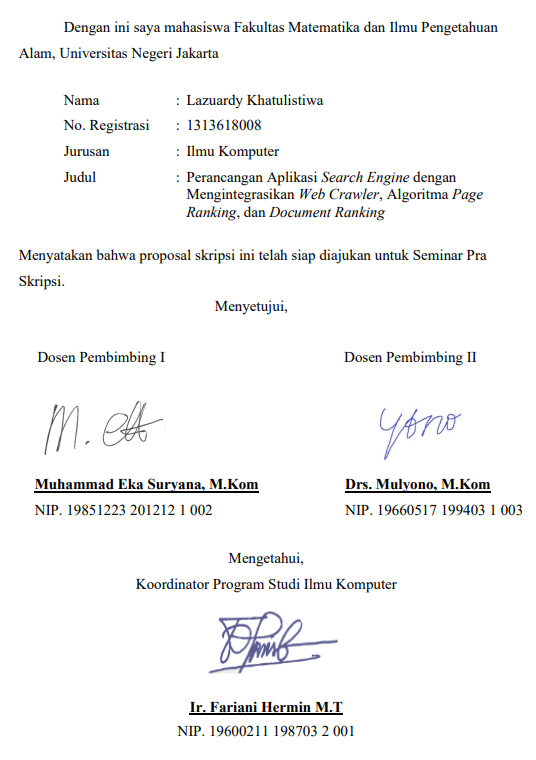
\includegraphics[keepaspectratio]{gambar/lembar_pengesahan}
\end{figure}
% \addcontentsline{toc}{chapter}{LEMBAR PENGESAHAN}
% \chapter*{\centering{\large{LEMBAR PERNYATAAN}}}

\begin{figure}[H]
	\centering
	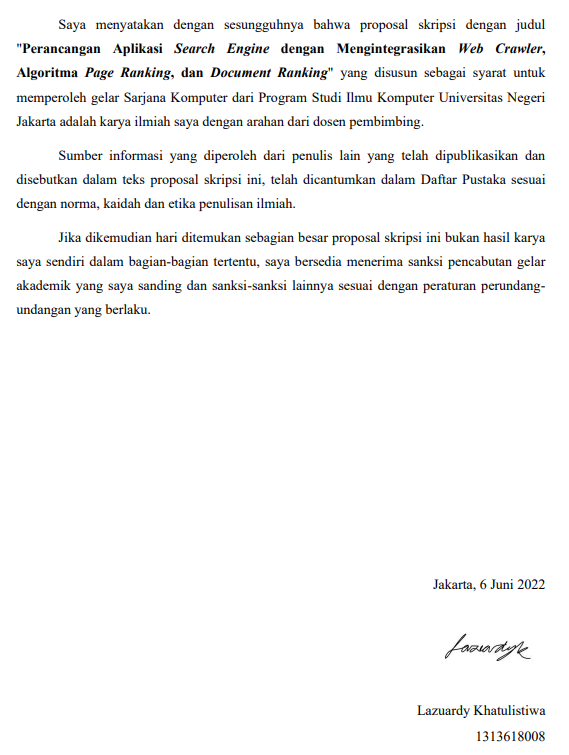
\includegraphics[keepaspectratio]{gambar/lembar_pernyataan}
\end{figure}
% \addcontentsline{toc}{chapter}{LEMBAR PERNYATAAN}
% \chapter*{\centering{\large{HALAMAN PERSEMBAHAN}}}
\null\vfill
\begin{flushright}
\textit{Untuk Keluargaku dan Diriku Sendiri.}
\end{flushright}
% \addcontentsline{toc}{chapter}{HALAMAN PERSEMBAHAN}
\chapter*{\centering{\large{KATA PENGANTAR}}}
 
\begin{spacing}{1.5}
	
Puji syukur penulis panjatkan ke hadirat Allah SWT, karena dengan rahmat dan karunia-Nya, penulis dapat menyelesaikan skripsi yang berjudul \textbf{"Ekspansi Aplikasi Aqua Breeding Dengan Penambahan Fitur Inventarisasi Untuk Penentuan Harga Dasar Produk Perikanan Berbasis Android"}.

Keberhasilan dalam menyusun skripsi ini tidak lepas dari bantuan berbagai pihak yang mana dengan tulus dan ikhlas memberikan masukan guna sempurnanya skripsi ini. Oleh karena itu dalam kesempatan ini, dengan kerendahan hati penulis mengucapkan banyak terima kasih kepada:

\begin{enumerate}

	\item{Yth. Para petinggi di lingkungan FMIPA Universitas Negeri Jakarta.}
	\item{Yth. Ibu Ria Arafiyah, M.Si selaku Koordinator Program Studi Ilmu Komputer.}
	\item{Yth. Bapak Muhammad Eka Suryana, M.Kom selaku Dosen Pembimbing I yang telah membimbing, mengarahkan, serta memberikan saran dan koreksi terhadap skripsi ini.}
	\item{Yth. Bapak Med Irzal, M.Kom selaku Dosen Pembimbing II yang telah membimbing, mengarahkan, serta memberikan saran dan koreksi terhadap skripsi ini.}
	\item{Yth. Seluruh Dosen Ilmu Komputer Universitas Negeri Jakarta yang telah mendidik dan mengarahkan dari sisi akademik dalam penyusunan skripsi ini.}
	\item{Orang tua penulis yang selama ini telah memberikan semengat, dukungan, serta doa kepada penulis dalam proses pembuatan skripsi ini.}
	\item{Teman-teman Program Studi Ilmu Komputer 2019 yang telah mendukung dan menjadi penyemangat penulis.}
	
\end{enumerate}

Penulis menyadari bahwa penyusunan skripsi ini masih jauh dari sempurna karena keterbatasan ilmu dan pengalaman yang dimiliki. Oleh karenanya, kritik dan saran yang bersifat membangun akan penulis terima dengan senang hati. Akhir kata, penulis berharap tugas akhir ini bermanfaat bagi semua pihak khususnya penulis sendiri. Semoga Allah SWT senantiasa membalas kebaikan semua pihak yang telah membantu penulis dalam menyelesaikan skripsi ini.

\end{spacing}

\vspace{2cm}

\begin{tabular}{p{8.5cm}c}
	&Jakarta, 02 Agustus 2023\\
	&\\
	&\\
	&\\
	&Akbar Maulana Alfatih
\end{tabular}
\addcontentsline{toc}{chapter}{KATA PENGANTAR}
\tableofcontents 
\addcontentsline{toc}{chapter}{DAFTAR ISI}
% \listoffigures
% \addcontentsline{toc}{chapter}{DAFTAR GAMBAR}
% \listoftables
% \addcontentsline{toc}{chapter}{DAFTAR TABEL}

\begin{counterpage}
\end{counterpage}
%Disini awal masukan untuk Bab
%-----------------------------------------------------------------
%!TEX root = ./template-skripsi.tex
%-------------------------------------------------------------------------------
% 								BAB I
% 							LATAR BELAKANG
%-------------------------------------------------------------------------------

\chapter{PENDAHULUAN}

\begin{spacing}{1.5}

\section{Latar Belakang Masalah}

Perikanan merupakan suatu sumber penghasilan terbesar yang ada di Indonesia dikarenakan Indonesia sendiri disebut sebagai negara maritim yang memiliki arti negara kepulauan. Oleh karena itu, banyak penduduk di Indonesia yang bermata pencaharian sebagai pembudidaya ikan. Namun, jika terlalu banyak menangkap ikan akan menyebabkan \textit{over fishing} yang membuat kemampuan bereproduksi ikan akan jauh lebih kecil daripada jumlah ikan hasil tangkapan. Hal ini akan menyebabkan langkanya spesies ikan tersebut dan berkurangnya angka produksi ikan. Dengan demikian, untuk mengatasi hal tersebut diperlukan budidaya perikanan yang berguna untuk menjaga ikan sampai masa panen tiba, serta dapat meningkatkan nilai ekonomi para pembudidaya ikan.

Dalam menjalankan budidaya perikanan, kebanyakan pembudidaya ikan masih melakukan cara manual dalam mengelola budidayanya. Hal ini tentunya kurang efektif dalam jangka panjang dan akan menyulitkan dalam pengelolaan budidayanya. Oleh karena itu, dalam penelitian yang dibuat oleh \citep{fishtalk} dan \citep{haucs} dapat berguna dalam menerapkan budidaya perikanan modern.

Yi-Bing Lin dan timnya membuat \textit{smart aquarium} yang bertujuan untuk meningkatkan kualitas akuarium yang bernama FishTalk. FishTalk memungkinkan sebuah sensor pada akuarium untuk menggerakan aktuator secara real time. Kegunaan dari \textit{smart aquarium} ini seperti sistem pemberian pakan otomatis dan pengendalian air dalam kolam secara otomatis. \citep{fishtalk}

Sementara itu, Bing Ouyang dan timnya membuat sebuah sistem yang dibentuk dan digunakan untuk monitoring serta \textit{decision making} pada tambak perikanan, sistem ini dinamakan HAUCS (\textit{Hybrid Aerial Underwater Robotic System}). Pemantauan ini dilakukan dengan memanfaatkan sistem robotik, mesin, dan operator manusia. Tujuan dibentuknya HAUCS ini adalah untuk meringankan pekerjaan manusia dari tugas yang berat, terlalu banyak biaya, dan memakan waktu dalam operasi pelaksanaan budidaya \textit{aquaculture} melalui platform pemanfaatan sistem robotik. \citep{haucs}

Dari kedua penelitian diatas, dapat disimpulkan bahwa alat yang digunakan dapat bermanfaat bagi para pembudidaya ikan karena dapat mempermudah pengelolaan budidaya. Namun, tentunya alat dan bahan yang dibutuhkan cukup banyak dan pasti mematok harga yang tidak sedikit. 

Oleh karena itu, penelitian yang dilakukan oleh \citep{waterquality} dan timnya mungkin dapat mengatasi masalah tersebut. Penelitian ini bertujuan untuk membuat big data dengan \textit{framework} SpringBoot dan Java Persistence API (JPA) yang didalamnya terdapat data kualitas air pada setiap perkembangbiakan ikan ternak. Platform ini dapat digunakan untuk memprediksi kualitas air dari setiap kolam dan memberikan notifikasi langsung ketika ada masalah pada kolam tersebut. Namun, penelitian ini hanya berfokus pada pendataan kualitas air saja sehingga rincian lain dari budidaya tersebut masih belum lengkap. \citep{waterquality} 

Tapi, tidak seperti dua penelitian yang sudah dirujuk sebelumnya, penelitian \citep{waterquality} ini berbasis aplikasi sehingga tidak ada biaya peralatan tambahan. Dengan demikian, pembudidaya ikan akan lebih terbantu jika terdapat aplikasi yang dapat membantu mereka dalam mengembangkan budidayanya tanpa perlu mengeluarkan biaya tambahan.

Pada penelitian yang dilakukan oleh \citep{fadhil2021}, \citep{gian2022} dan \citep{andri2022}, mereka membuat suatu aplikasi bernama \textit{Aqua Breeding} yang berfungsi untuk mencatat pendetailan dari setiap budidaya para pembudidaya ikan. Detail yang dimaksud seperti pencatatan pakan ikan, pencatatan angka kematian ikan, pengendalian kualitas air, dan pencatatan lainnya yang berhubungan pada musim budidaya ikan tersebut. Aplikasi ini tentunya dapat membantu para pembudidaya ikan dan juga dapat meningkatkan ekonomi pembudidaya ikan sejalan dengan lancarnya musim budidaya.

Penelitian yang terkait dalam aplikasi tersebut adalah penelitian Fadhil Perwira Hadi yang berjudul “Rancang Bangun Web Service dan Website sebagai Storage Engine dan Monitoring Data Sensing untuk Budidaya Ikan Air Tawar” menghasilkan suatu sistem web service yang dapat menerima data yang dikirimkan oleh \textit{embedded device}, dengan menerapkan konsep IoT \citep{fadhil2021}. \textit{Web service} tersebut kemudian dilanjutkan dengan penelitian Andri Rahmanto dengan judul “Perancangan Arsitektur Aplikasi Budidaya Perikanan Modern pada Backend yang bertanggung jawab dalam melayani Transaksi Query Webservice dengan menggunakan Teknologi Flask Microservice”. \textit{Web service} ini menghasilkan \textit{output} berupa arsitektur aplikasi budidaya perikanan modern pada \textit{backend} berupa \textit{endpoint} yang dapat digunakan untuk pendataan budidaya perikanan air tawar \citep{andri2022}. Dalam pengolahan \textit{backend} ini, Gian Chiesa Maghriza dengan penelitiannya yang berjudul “Perancangan Frontend Aplikasi Pendukung Teknologi Perikanan Modern dengan menggunakan Framework Flutter yang mentarget Multi Platform” membuat \textit{user interface} serta konfigurasi fitur pencatatan dari aplikasi teknologi perikanan modern. Fitur-fitur yang ada pada aplikasi ini didasari pada penggunaan \textit{endpoint} yang sudah disediakan pada \textit{backend} buatan Andri \citep{gian2022}. Namun pada aplikasi tersebut masih terdapat kekurangan seperti belum tersedia fitur inventarisasi sebagai \textit{storage} dalam berbudidaya.

Hal tersebut tentunya masih belum memecahkan masalah dari pembudidaya ikan dalam menjalankan budidayanya. Masalah yang paling berdampak pada pembudidaya ikan adalah saat harga komoditas mengalami kenaikan sedangkan harga jual ikan tidak mengalami perubahan dikarenakan harga yang sudah ditetapkan oleh Kemendagri sehingga pembudidaya ikan bisa mengalami kerugian. Hal ini tentunya akan membawa dampak negatif dalam nilai ekonomi perikanan.

Oleh karena itu, penelitian ini bertujuan untuk memecahkan masalah tersebut dengan menambahkan sistem inventarisasi pada aplikasi \textit{Aqua Breeding} ini untuk menentukan harga dasar pada produk perikanan. Dengan demikian, harga dasar tersebut dapat digunakan oleh pembudidaya ikan untuk penjualan hasil panen mereka. Selain itu, fitur inventarisasi ini juga dapat membantu para pembudidaya ikan dalam mengolah dan mengontrol kebutuhan serta pengeluaran dalam setiap musim budidaya. Berdasarkan fitur baru yang sudah dijelaskan sebelumnya, aplikasi ini diharapkan dapat membantu para pembudidaya ikan untuk berbudidaya dalam hal penentuan harga dasar dan pengendalian kebutuhan saat budidaya berlangsung. 

\section{Rumusan Masalah}
Dari uraian latar belakang di atas, perumusan masalah pada penelitian ini ialah “Bagaimana rancangan sistem inventaris yang digunakan untuk menentukan harga dasar dan harga jual minimum dari produk perikanan berbasis Android?”.

\section{Pembatasan Masalah}
Pembatasan masalah pada penelitian ini antara lain:
\begin{enumerate}
	\item Aplikasi hanya menentukan harga jual minimum dari produk perikanan.
\end{enumerate}

\section{Tujuan Penelitian}
	Penelitian ini dilakukan dengan tujuan untuk membuat aplikasi perikanan berbasis Android dengan sistem inventaris untuk menentukan harga jual minimum dari produk perikanan.

\section{Manfaat Penelitian}
\begin{enumerate}
	\item Bagi penulis
		
	Meningkatkan pengetahuan sistem inventaris pada produk perikanan, menambah pengalaman dalam mengembangkan aplikasi, memperoleh gelar sarjana di bidang Ilmu Komputer, serta menjadi media untuk penulis dalam mengaplikasikan ilmu yang didapat dari kampus.
		
	\item Bagi Universitas Negeri Jakarta
	 	
	Menjadi pedoman untuk penelitian di masa depan, dan dapat memberikan panduan bagi mahasiswa program studi Ilmu Komputer tentang penentuan harga dasar pada produk perikanan dengan sistem inventaris.
	
	\item Bagi masyarakat
	 	
	Membantu masyarakat yang ingin dan sedang menggeluti bidang budidaya perikanan dalam proses penentuan harga dasar pada produk perikanan.
	 			
\end{enumerate}


% Baris ini digunakan untuk membantu dalam melakukan sitasi
% Karena diapit dengan comment, maka baris ini akan diabaikan
% oleh compiler LaTeX.
\begin{comment}
\bibliography{daftar-pustaka}
\end{comment}

\end{spacing}
 %!TEX root = ./template-skripsi.tex
%-------------------------------------------------------------------------------
%                            BAB II
%               KAJIAN TEORI
%-------------------------------------------------------------------------------

\chapter{KAJIAN PUSTAKA} 

\section{Pengertian Persediaan dan Manajemen Persediaan}

Pada buku Dasar-Dasar Manajemen \citep{dasarmanajemen}, dijelaskan bahwa persediaan adalah sebuah stok aset yang dimiliki oleh perusahaan. Aset ini dapat berupa bahan mentah, bahan baku, barang jadi, barang dalam proses, hingga bahan pembantu. Persediaan merupakan aset yang berharga, karena berkaitan dengan proses produksi. Persediaan yang tidak teratur dapat menyebabkan kerugian, sehingga menerapkan manajemen persediaan dalam suatu bisnis merupakan hal yang penting. 

Manajemen persediaan merupakan suatu cara untuk melakukan pengawasan, kontrol, pengelolaan terhadap persediaan yang dimiliki oleh perusahaan. Berbagai macam kegiatan yang berkaitan dengan memperoleh, menyimpan, hingga menggunakan persediaan merupakan bagian dari manajemen persediaan.

Manajemen persediaan memiliki beberapa fungsi, yaitu:
\begin{enumerate}
	\item Mencegah terjadinya kekurangan persediaan.
	\item Mencegah barang dari supplier tidak sesuai kebutuhan.
	\item Memastikan proses produksi berjalan dengan lancar.
	\item Mengantisipasi permintaan yang mendadak.
	\item Menyesuaikan pembelian dengan jadwal produksi.
\end{enumerate}

Selain beberapa fungsi yang sudah disebutkan diatas, Manajemen persediaan juga memiliki tujuan. Beberapa tujuan dari manajemen persediaan adalah sebagai berikut.
\begin{enumerate}
	\item Mengantisipasi kenaikan harga bahan baku.
	\item Memastikan persediaan selalu tersedia.
	\item Mengurangi resiko bahan baku yang datang terlambat.
	\item Menjaga jumlah persediaan tetap stabil.
	\item Mengantisipasi kemungkinan adanya perubahan dari segi penawaran ataupun permintaan.
\end{enumerate}

\section{Jenis-jenis Manajemen Persediaan}

Manajemen persediaan dibagi menjadi beberapa jenis, diantaranya:

\begin{enumerate}
	\item Bahan Mentah
	
	Bahan mentah atau bahan baku merupakan bahan utama atau dasar dari dibuatnya suatu produk. Tanpa adanya bahan baku, maka produk tidak bisa masuk ke tahap produksi. Oleh karena itu manajemen persediaan diperlakukan untuk mengelola bahan baku agar selalu tersedia dan siap untuk diproses.
	
	\item Barang Setengah Jadi
	
	Barang setengah jadi atau barang dalam proses merupakan barang yang belum sepenuhnya bisa digunakan, sehingga perlu untuk diproses lebih lanjut untuk menjadi barang jadi, yang nantinya siap untuk digunakan. Dalam hal ini, manajemen persediaan digunakan untuk menghitung banyaknya barang setengah jadi tersebut untuk memenuhi kebutuhan pasar.

	\item Barang Jadi
	
	Barang jadi merupakan barang yang sudah siap untuk dijual. Manajemen persediaan berguna untuk mengatur pengiriman barang tersebut ke pasar sehingga keadaan produk di pasar tetap stabil.
\end{enumerate}

\section{Biaya Persediaan}

Penetapan biaya persediaan atau evaluasi persediaan memungkinkan perusahaan untuk memberikan nilai moneter untuk barang-barang dalam persediaan mereka. Inventaris perusahaan seringkali merupakan aset terbesarnya dan pengukuran yang tepat untuk memastikan keakuratan laporan keuangan.

Untuk menentukan biaya persediaan, diperlukan lima langkah-langkah sebagai berikut.

\begin{enumerate}
	\item Menentukan periode waktu tertentu yang dimana perlu menemukan nilai inventaris.
	\item Memastikan persediaan selalu tersedia.
	\item Mengurangi resiko bahan baku yang datang terlambat.
	\item Menjaga jumlah persediaan tetap stabil.
	\item Mengantisipasi kemungkinan adanya perubahan dari segi penawaran ataupun permintaan.
\end{enumerate}

% Pada buku Pengendalian Persediaan \citep{pengendalianpersediaan}, dijelaskan bahwa terdapat beberapa metode yang digunakan untuk menentukan biaya persediaan, antara lain:

% \subsection{Metode identifikasi khusus (\textit{Specific Identification Method})}

% Dalam metode ini, setiap jenis barang yang ada di gudang harus diberi tanda sesuai dengan harga pokok per satuan barang tersebut dibeli. Jika terdapat barang yang harga satuannya berbeda dengan harga satuan barang yang ada di gudang, maka harus dipisahkan penyimpanannya dan diberi tanda pada harga berapa barang tersebut dibeli.

% Masalah yang ada pada metode ini terletak dalam penyimpanan barang di gudang. Meskipun jenis barangnya sama, namun jika harga pokok per satuannya berbeda maka barang tersebut harus disimpan secara terpisah agar mudah diidentifikasi saat pemakaian nanti.

% \subsection{Metode FIFO (\textit{First-in, First-out})}

% Metode FIFO merupakan metode penentuan biaya persediaan dengan anggapan bahwa harga pokok per satuan barang yang pertama masuk dalam gudang digunakan untuk menentukan harga barang yang pertama kali dipakai. Sebagai contoh dapat dilihat perhitungan berikut.

% Data mengenai barang saat minggu pertama bulan Januari 2020 sebagai berikut.

% 	\begin{table}[H]	
% 		\begin{center}
% 			\caption{Data tabel pada barang bulan Januari 2020}
% 			\label{tab:table1}
% 			\begin{tabular}{c|c} % <-- Alignments: 1st column left, 2nd middle and 3rd right, with vertical lines in between
% 			\textbf{Tanggal} & \textbf{Deskripsi} \\
% 			\hline
% 			01 Januari 2020 & Persediaan 8,000 kg dengan harga Rp1.000,00/kg \\
% 			08 Januari 2020 & Melakukan pembelian barang sebesar 12,000 kg \\
% 			&  dengan harga Rp1.200,00/kg \\
% 			09 Januari 2020 & Masuk proses produksi sebanyak 15,000 kg \\
% 			\end{tabular}
% 		\end{center}
% 	\end{table}

% Barang yang masuk pertama yaitu barang yang pertama kali digunakan dalam proses produksi. Berdasarkan data pada tabel diatas, dapat dihitung biaya persediaannya dengan cara dibawah ini. 

% 8,000 kg $\times$ Rp1.000,00 = Rp8.000.000,00

% 7,000 kg $\times$ Rp1.200,00 = Rp8.400.000,00

% Total = 15.000 kg = Rp16.400.000,00

% \textbf{Biaya Persediaan akhir} = 5.000 kg $\times$ Rp1.200,00 = Rp6.000.000,00

% \subsection{Metode LIFO (\textit{Last-in, Last-out})}

% Metode LIFO merupakan metode penentuan biaya persediaan dengan anggapan bahwa harga pokok per satuan barang yang terakhir masuk dalam persediaan dipakai untuk menentukan harga pokok barang yang pertama kali dipakai dalam produksi. Sebagai contoh dapat dilihat perhitungan dengan data tabel yang sama.

% Barang yang terakhir masuk merupakan barang yang digunakan terlebih dahulu dalam proses produksi.

% 12,000 kg $\times$ Rp1.200,00 = Rp14.400.000,00

% 3,000 kg $\times$ Rp1.000,00 = Rp3.000.000,00

% Total = 15.000 kg = Rp17.400.000,00

% \textbf{Biaya Persediaan akhir} = 5.000 kg $\times$ Rp1.000,00 = Rp5.000.000,00

% \subsection{Metode rata-rata bergerak (\textit{Moving Average Method})}

% Dalam metode ini, persediaan barang yang ada digudang dihitung harga pokok rata-ratanya dengan cara membagi total pokok dengan jumlah satuannya. Metode ini disebut juga rata-rata tertimbang, karena dalam menghitung rata-rata harga pokok persediaan barang, metode ini menggunakan kuantitas barang sebagai angka penimbangnya. Sebagai contoh dapat dilihat perhitungan dibawah dengan tabel yang sama seperti sebelumnya.

% Biaya barang yang dipakai dalam proses produksi yaitu hasil kali kuantitas barang yang dipakai dan harga rata-rata per satuan.

% 8,000 kg $\times$ Rp1.000,00 = Rp8.000.000,00

% 12,000 kg $\times$ Rp1.200,00 = Rp14.000.000,00

% Total = 20.000 kg = Rp22.400.000,00

% Harga rata-rata = Rp22.400.000,00 : 20.000 kg = Rp1.120,00

% Total = 15.000 kg $\times$ Rp1.120,00 = Rp16.800.000,00

% \textbf{Biaya Persediaan akhir} = 5.000 kg $\times$ Rp1.120,00 = Rp5.600.000,00

% \subsection{Metode biaya standar}

% Pada metode ini, barang yang dibeli dicatat dalam kartu persediaan sebesar harga standar yaitu harga taksiran yang mencerminkan harga yang diharapkan akan terjadi dimasa yang akan datang. Harga standar merupakan harga yang diperkirakan untuk tahun tertentu.

% \subsection{Metode rata-rata harga pokok bahan pada akhir bulan}

% Dengan metode ini, pada akhir bulan dilakukan perhitungan harga pokok rata-rata per satuan tiap jenis persediaan barang yang ada digudang. Harga pokok rata-rata per satuan kemudian digunakan untuk menghitung harga pokok barang yang dipakai dalam produksi bulan berikutnya.

% \subsection{First In, First Out (FIFO)} 
	
% 	\textit{First-in, first-out} atau FIFO adalah metode dimana aset yang diproduksi dan diperoleh terlebih dahulu juga dijual atau digunakan terlebih dahulu. Saat menggunakan FIFO sebagai metode pilihan, gunakan perhitungan ini untuk menentukan harga pokok penjualan (HPP)-nya:
% 	\begin{equation}
% 		\begin{split}
% 			HPP
% 			&= Biaya\;persediaan\;terlama \times Jumlah\;persediaan\;yang\;terjual
% 		\end{split}
% 	\end{equation}

% 	\textbf{Contoh FIFO} : 

% 	\begin{table}[H]
% 		\begin{center}
% 		  \caption{Data tabel dalam persediaan barang}
% 		  \label{tab:table1}
% 		  \begin{tabular}{l|c|r} % <-- Alignments: 1st column left, 2nd middle and 3rd right, with vertical lines in between
% 			\textbf{Tanggal} & \textbf{Deskripsi} & \textbf{Unit dan Biaya} \\
% 			\hline
% 			1 Maret & Inventaris awal & 65 unit, \${15} per unit\\
% 			5 Maret & Beli &  130 unit, \${10} per unit\\
% 			10 Maret & Jual &  95 unit, \${20} per unit\\
% 			12 Maret & Beli &  35 unit, \${15} per unit\\
% 			15 Maret & Beli &  75 unit, \${20} per unit\\
% 			21 Maret & Jual &  115 unit, \${30} per unit\\
% 			28 Maret & Jual &  60 unit, \${35} per unit\\
% 		  \end{tabular}
% 		\end{center}
% 	  \end{table}
% 	  \begin{enumerate}
% 		\item \textbf{Tentukan jumlah unit yang tersedia untuk dijual}
		
% 		Tentukan jumlah unit yang tersedia untuk dijual dengan menjumlahkan semua unit beli dengan inventaris awal.

% 		\textbf{Unit yang tersedia untuk dijual = 65 + 130 + 35 + 75}

% 		\textbf{Unit yang tersedia untuk dijual = 305}

% 		Terdapat 305 unit yang tersedia untuk dijual.

% 		\item \textbf{Tentukan jumlah unit yang dijual}
		
% 		Tentukan jumlah unit yang dijual dengan menjumlahkan semua unit yang dijual.

% 		\textbf{Unit dijual = 95 + 115 + 60}

% 		\textbf{Unit dijual = 270}

% 		Ada 270 unit yang dijual.

% 		\item \textbf{Tentukan nilai inventaris akhir}
		
% 		Tentukan nilai inventaris akhir dengan cara mengurangi jumlah unit yang tersedia untuk dijual dengan jumlah unit yang dijual.

% 		\textbf{Inventaris akhir = Jumlah unit yang tersedia untuk dijual - jumlah unit yang dijual}

% 		\textbf{Inventaris akhir = 305 - 270}

% 		\textbf{Inventaris akhir = 35}

% 		Ada 35 unit yang tersisa pada inventaris akhir.

% 		\item \textbf{Menentukan HPP menggunakan rumus FIFO}
		
% 		Biaya persediaan terlama dapat ditentukan dengan nilai inventaris awal. Nilai tersebut didapat dengan mengalikan persediaan awal dan harga per unitnya. 

% 		\textbf{HPP = biaya persediaan terlama $\times$ jumlah persediaan yang dijual}

% 		\textbf{HPP = (65 $\times$ 15) $\times$ 270}

% 		\textbf{HPP = 263,250}

% 		Biaya barang yang dijual adalah \${263,250}.

% 	  \end{enumerate}

% \subsection{Last In, First Out (LIFO)}
	
% 	\textit{Last-in, first-out} atau LIFO adalah metode yang mencatat barang-barang yang baru saja diproduksi sebagai barang yang terjual lebih dulu. Saat menggunakan LIFO sebagai metode pilihan, gunakan perhitungan ini untuk menentukan harga pokok penjualan (HPP)-nya:
% 	\begin{equation}
% 		\begin{split}
% 			HPP
% 			&= Biaya\;persediaan\;terakhir \times Jumlah\;persediaan\;yang\;terjual
% 		\end{split}
% 	\end{equation}

% 	\textbf{Contoh LIFO} :

% 	\begin{table}[H]
% 		\begin{center}
% 		  \caption{Data tabel dalam persediaan barang}
% 		  \label{tab:table2}
% 		  \begin{tabular}{l|c|r} % <-- Alignments: 1st column left, 2nd middle and 3rd right, with vertical lines in between
% 			\textbf{Tanggal} & \textbf{Deskripsi} & \textbf{Unit dan Biaya} \\
% 			\hline
% 			3 April & Inventaris awal & 70 unit, \${15} per unit\\
% 			6 April & Beli &  125 unit, \${10} per unit\\
% 			10 April & Beli &  90 unit, \${20} per unit\\
% 			13 April & Jual &  40 unit, \${15} per unit\\
% 			16 April & Beli &  50 unit, \${15} per unit\\
% 			23 April & Jual &  100 unit, \${20} per unit\\
% 			29 April & Jual &  70 unit, \${20} per unit\\
% 		  \end{tabular}
% 		\end{center}
% 	  \end{table}

% 	\begin{enumerate}
% 		\item \textbf{Menentukan biaya persediaan terbaru}
		
% 		Untuk mencari biaya persediaan terbaru dapat dilakukan dengan menggunakan data pada inventaris awal.

% 		\textbf{Biaya persediaan terbaru = 70 $\times$ 15}

% 		\textbf{Biaya persediaan terbaru = 1,050}

% 		Biaya persediaan terbaru adalah \${1,050}.

% 		\item \textbf{Temukan jumlah unit yang dijual}
		
% 		Temukan jumlah unit yang terjual dengan menambahkan semua unit yang dijual.

% 		\textbf{Jumlah unit yang dijual = 40 + 100 + 70}

% 		\textbf{Jumlah unit yang dijual = 210}

% 		Ada 210 unit yang dijual.

% 		\item Gunakan rumus LIFO
		
% 		Gunakan biaya persediaan terbaru dan total unit yang dijual untuk menentukan nilai HPP-nya.

% 		\textbf{HPP = biaya persediaan terbaru $\times$ jumlah persediaan yang dijual}

% 		\textbf{HPP = 1,050 $\times$ 210}

% 		\textbf{HPP = 220,500}

% 		Biaya barang yang dijual adalah \${220,500}.

% 	\end{enumerate}

% 	\subsection{Rata-rata tertimbang}
	
% 	Rata-rata tertimbang atau biaya rata-rata tertimbang yang biasa dikenal sebagai \textit{Weighted Average Cost} (WAC) adalah metode yang menentukan jumlah masuk ke HPP dan persediaan melalui penggunaan rata-rata tertimbang. Saat menggunakan WAC, gunakan perhitungan ini:
% 	\begin{equation}
% 		\begin{split}
% 			WAC\;per\;unit
% 			&= Harga\;pokok\;barang\;yang\;tersedia \div unit\;yang\;tersedia
% 		\end{split}
% 	\end{equation}

% 	\textbf{Contoh WAC} :
% 	\begin{table}[H]
% 		\begin{center}
% 		  \caption{Data tabel dalam persediaan barang}
% 		  \label{tab:table3}
% 		  \begin{tabular}{l|c|r} % <-- Alignments: 1st column left, 2nd middle and 3rd right, with vertical lines in between
% 			\textbf{Tanggal} & \textbf{Deskripsi} & \textbf{Unit dan Biaya} \\
% 			\hline
% 			3 Mei & Inventaris awal & 30 unit, \${15} per unit\\
% 			6 Mei & Beli &  50 unit, \${15} per unit\\
% 			11 Mei & Jual &  25 unit, \${25} per unit\\
% 			15 Mei & Jual &  30 unit, \${10} per unit\\
% 			18 Mei & Beli &  15 unit, \${25} per unit\\
% 			22 Mei & Beli &  25 unit, \${35} per unit\\
% 			25 Mei & Jual &  35 unit, \${30} per unit\\
% 		  \end{tabular}
% 		\end{center}
% 	  \end{table}

% 	\begin{enumerate}
% 		\item Tentukan biaya setiap penjualan
		
% 		Menentukan biaya setiap penjualan dengan menghitung harga dari masing-masing semua unit yang dijual.

% 		\textbf{Penjualan tanggal 11 Mei} = 25 $\times$ 25 = \textbf{\${625}}

% 		\textbf{Penjualan tanggal 15 Mei} = 30 $\times$ 10 = \textbf{\${300}}

% 		\textbf{Penjualan tanggal 25 Mei} = 35 $\times$ 30 = \textbf{\${1,050}}

% 		\item Menjumlahkan semua biaya setiap penjualan
		
% 		Menggabungkan semua biaya setiap penjualan dari unit yang dijual.

% 		\textbf{Harga pokok barang yang tersedia = 625 + 300 + 1,050}

% 		\textbf{Harga pokok barang yang tersedia = \${1,975}}

% 		\item Temukan unit yang tersedia untuk dijual
		
% 		Totalkan semua unit yang tersedia untuk dijual dengan inventaris awal.

% 		\textbf{Unit yang tersedia untuk dijual = 30 + 50 + 15 + 25}

% 		\textbf{Unit yang tersedia untuk dijual = 120 unit}

% 		\item Gunakan rumus rata-rata tertimbang
		
% 		\textbf{WAC per unit = harga pokok barang yang tersedia / unit yang tersedia}
		
% 		\textbf{WAC per unit = 1,975 / 120}
		
% 		\textbf{WAC per unit = \${16.49}}

% 		Dari perhitungan tersebut, didapat biaya rata-rata tertimbang atau WAC-nya adalah \${16.49}
% 	\end{enumerate}

% \section{EOQ}

% \textit{Economic order quantity} (EOQ) merupakan jumlah persediaan yang digunakan untuk meminimalkan jumlah dan biaya pemesanan yang terkait dengan bahan baku atau persediaan barang dagangan. Intinya, EOQ merupakan \textit{set point} yang dibuat dan digunakan untuk menjadi acuan dalam membantu perusahaan meminimalkan total biaya persediaan.

% Dua faktor penting yang menjadi penentu dalam menentukan \textit{economic order quantity} (EOQ) adalah biaya pemesanan dan biaya penyimpanan.

% \begin{enumerate}
% 	\item Biaya pemesanan
	
% 	Biaya pemesanan merupakan biaya yang dikeluarkan setiap pesanan. Contoh hal yang termasuk biaya pemesanan adalah biaya pengiriman, biaya pemrosesan pembayaran, dan lain-lain.

% 	\item Biaya persediaan
	
% 	Biaya persediaan merupakan biaya yang dikeluarkan untuk menyimpan persediaan di toko atau gudang. Contoh hal yang termasuk dalam biaya penyimpanan adalah biaya sewa ruang penyimpanan, pajak properti, dan lain-lain.
% \end{enumerate}

% Formula atau rumus yang digunakan untuk menentukan EOQ adalah:

% \begin{equation}
%     \begin{split}
% 		EOQ
% 		&= \sqrt{\frac{2 \times D \times Co}{Ch}}
%     \end{split}
% \end{equation}

% \begin{itemize}
% 	\item D = \textit{Demand per year} (Kebutuhan per tahun)
% 	\item Co = \textit{Cost per order} (Biaya per pesanan)
% 	\item Ch = \textit{Cost of holding per unit of inventory} (Biaya persediaan per unit)
% \end{itemize}

% \textbf{Contoh Kasus}

% Sebuah material DX digunakan rutin setiap tahunnya. Data kebutuhan per tahun, biaya pemesanan, dan biaya persediaan per unit adalah sebagai berikut.

% \begin{itemize}
% 	\item Kebutuhan tahunan = 2,400 unit
% 	\item Biaya per pesanan = \${10} per pesanan
% 	\item Biaya persediaan per unit = \${0.30} per unit
% \end{itemize}

% Diketahui:
% \begin{itemize}
% 	\item D = \textit{Demand per year} (Kebutuhan per tahun) -> 2,400
% 	\item Co = \textit{Cost per order} (Biaya per pesanan) -> \${10}
% 	\item Ch = \textit{Cost of holding per unit of inventory} (Biaya persediaan per unit) -> \${0.30}
% \end{itemize}

% Maka, EOQ-nya adalah sebagai berikut.

% \begin{equation}
%     \begin{split}
% 		EOQ
% 		&= \sqrt{\frac{2 \times D \times Co}{Ch}} \\
% 		&= \sqrt{\frac{2 \times 2,400 \times 10}{0.30}} \\
% 		&= \sqrt{\frac{48,000}{0.30}} \\
% 		&= \sqrt{160,000} \\
% 		&= 400
%     \end{split}
% \end{equation}

% Dapat dilihat bahwa EOQ dari material DX adalah sebesar 400 unit. Sekarang dapat dihitung berapa jumlah penjualan tahunan, biaya pemesanan tahunan, biaya penyimpanan tahunan, dan juga kombinasi dari biaya pemesanan tahunan dan biaya persediaan tahunan sebagai berikut.

% \textbf{Jumlah penjualan tahunan}

% = Kebutuhan tahunan / EOQ

% = 2,400 unit / 400 unit

% = 6 pesanan per tahun

% \textbf{Biaya pemesanan tahunan}

% = Jumlah penjualan tahunan * Biaya pemesanan per unit

% = 6 pesanan * \${10}

% = \${60}

% \textbf{Biaya penyimpanan tahunan}

% = Rata-rata unit * Biaya penyimpanan

% = (400/2) * 0.3

% = \${60}

% \textbf{Kombinasi antara biaya pemesanan dan biaya penyimpanan}

% = Biaya pemesanan tahunan + biaya penyimpanan tahunan

% = \${60} + \${60}

% = \${120}

% \begin{table}[h!]
% 	\caption{Tabel Hasil Perhitungan EOQ}
% 	\label{tab:table2}
% 	\begin{tabular}{|m{0.1\linewidth}|m{0.1\linewidth}|m{0.13\linewidth}|m{0.13\linewidth}|m{0.16\linewidth}|m{0.13\linewidth}|} % <-- Alignments: 1st column left, 2nd middle and 3rd right, with vertical lines in between
% 	\hline
% 	\multicolumn{1}{|c|}{Jumlah Pesanan} & \multicolumn{1}{|c|}{Nilai} & \multicolumn{1}{|c|}{Rata-rata barang} & \multicolumn{3}{c|}{Biaya Pemesanan dan Penyimpanan} \\
% 	\cline{4-6}
% 	\multicolumn{1}{|c|}{Per Tahun} & \multicolumn{1}{|c|}{EOQ} & \multicolumn{1}{|c|}{dalam Persediaan} & Biaya Pemesanan & Biaya Penyimpanan & Biaya Gabungan \\
% 	\hline
% 		1 & 2,400 & 1,200 & 10 & 360 & 370\\ \hline
% 		2 & 1,200 & 600 & 20 & 180 & 200\\ \hline
% 		3 & 800 & 400 & 30 & 120 & 150\\ \hline
% 		4 & 600 & 300 & 40 & 90 & 130\\ \hline
% 		5 & 480 & 240 & 50 & 72 & 122\\ \hline
% 		\textbf{6} & \textbf{400} & \textbf{200} & \textbf{60} & \textbf{60} & \textbf{120}\\ \hline
% 		7 & 343 & 172 & 70 & 52 & 122\\ \hline
% 		8 & 300 & 150 & 80 & 45 & 125\\ \hline
% 	\end{tabular}
% \end{table}


% Pada Tabel 2.4, dapat dilihat bahwa dengan data yang sama menghasilkan hitungan yang berbeda tergantung dari berapa banyak jumlah penjualan tahunannya.

% Dari hitungan EOQ yang sudah dilakukan sebelumnya, jumlah penjualan tahunan sebesar 6 pesanan per tahun mendapatkan biaya kombinasi yang lebih sedikit dan stabil dibandingkan dengan kurang atau lebih dari 6 pesanan per tahunnya. Hal ini dikarenakan jika semakin kecil angka penjualan tahunannya maka hal tersebut akan berdampak pada tingginya biaya penyimpanan yang menyebabkan ketidakseimbangan antara biaya pemesanan dan biaya penyimpanan. Sementara itu, jika penjualan pertahunnya itu tinggi maka hal tersebut akan berdampak pada tingginya biaya pemesanan yang menyebabkan hal yang serupa. Jadi, dapat disimpulkan bahwa perhitungan EOQ ini bersifat konstan terhadap biaya pemesanan dan biaya penyimpanan.

% Dari kesimpulan diatas, ada beberapa hal yang harus diperhatikan dalam penggunaan metode EOQ ini, yaitu:

% \begin{enumerate}
% 	\item Jumlah kebutuhan barang per periode stabil
% 	\item Hanya ada dua macam biaya yang relevan, yaitu biaya pemesanan dan biaya penyimpanan
% 	\item Biaya pemesanan selalu sama
% 	\item Biaya penyimpanan per unit selalu sama
% 	\item Usia barang tidak cepat rusak
% 	\item Harga barang tetap
% 	\item Barang tersedia tak terbatas.
% \end{enumerate}

% \section{ROP}

% Pada buku Pengendalian Persediaan \citep{pengendalianpersediaan}, dijelaskan bahwa dalam EOQ ditentukan titik pemesanan kembali atau \textit{reorder point} yang biasa dikenal sebagai (ROP), yaitu jumlah persediaan tetap setiap kali pemesanan. ROP dilakukan bila persediaan bisa memenuhi kebutuhan produksi selama masa tenggang waktu pemesanan. ROP menghendaki pengecekan kartu catatan secara teratur.

% Untuk menentukan waktu pemesanan kembali atau \textit{reorder point} dapat dilakukan dengan rumus berikut.

% \begin{equation}
%     \begin{split}
% 		ROP
% 		&= LT \times AU + SS
%     \end{split}
% \end{equation}

% \begin{itemize}
% 	\item ROP = \textit{Reorder point}, yaitu tingkat dimana perusahaan harus memesan kembali. 
% 	\item LT = \textit{Leadtime}, yaitu masa kadaluarsa antara pemesanan sampai dengan kedatangan bahan.
% 	\item AU = \textit{Average usage}, yaitu pemakaian rata-rata dalam pemakaian tertentu.
% 	\item SS = \textit{Safety stok} yaitu besarnya persediaan atau bisa dibilang \textit{minimum inventory point}.
% \end{itemize}

% Dalam menutupi kebutuhan persediaan, hal yang perlu dilakukan adalah pemesanan bahan. Pemesanan bahan yang diperlukan pada saat persediaan mencapai titik tertentu (\textit{order point system}) dan pemesanan yang diperlukan pada saat waktu tertentu yang sudah ditetapkan telah tercapai (\textit{order cycle system}).

% \subsection{Order Point System} 
	

% 	\textit{Order point system} adalah suatu sistem dimana pesanan dilakukan apabila persediaan yang ada telah mencapai tingkat tertentu. Jadi dengan sistem ini, ditentukan jumlah persediaan pada tingkatan tertentu yang merupakan batas tenggat waktu dilakukannya pemesanan yang disebut \textit{reorder point}. Dalam sistem ini, pesanan yang jumlahnya tetap dari bahan-bahan yang dipesan disebut dengan \textit{fixed order quantity system}. 

% 	Keuntungan dari sistem ini adalah pemantauan jumlah dan waktu pemesanan dapat dilakukan dengan mudah dan cepat.

% 	Dalam pelaksanaan sistem ini, dapat dilakukan dua variasi sebagai berikut.

% 	\begin{enumerate}
% 		\item \textit{Two bin and bag account system}
		
% 		Dengan cara ini, dapat digunakan dua kantong atau \textit{bin} dimana kantong pertama merupakan tempat persediaan bahan yang jumlahnya sama dengan jumlah persediaan pada tingkat \textit{order point} dan berfungsi sebagai persediaan cadangan. Sedangkan persediaan bahan-bahan selebihnya ditempatkan pada kantong kedua.

% 		Penggunaan bahan-bahan dimulai dari kantong kedua sampai habis dan ketika kantong kedua sudah habis maka diharuskan untuk melakukan pemesanan kembali.

% 		Sistem ini adalah sistem yang sederhana dan mudah untuk dilakukan pengendalian bahan ataupun pencatatan.

% 		\item \textit{One storage bin system}
		
% 		Dengan cara ini, hanya menggunakan satu kantong persediaan. Didalam kantong persediaan ini diadakan pembagian persediaan menjadi dua bagian. Bagian pertama dibagi untuk memenuhi kebutuhan bahan-bahan sehari-hari, sementara bagian kedua digunakan untuk memenuhi kebutuhan bahan-bahan selama periode pengisian kembali.

% 		Cara ini memberikan keuntungan berupa kesederhanaan dalam pencatatan persediaan.
% 	\end{enumerate}

% \subsection{Order Cycle System}
	
% 	\textit{Order cycle system} adalah sistem pemesanan bahan yang dimana jarak antara pemesanan tetap, sebagai contoh tiap minggu atau tiap bulan. Jadi, dengan sistem ini ditentukan waktu pemesanan dengan jarak yang konstan. Karena didasarkan pada jarak waktu yang konstan, maka pemesanan dilakukan tanpa memperhatikan jumlah persediaan yang masih ada. \textit{Order cycle system} dapat digunakan untuk memantau persediaan barang yang mempunyai banyak jenis.

% 	Sistem ini termasuk salah satu sistem yang kaku dan mahal, karena setiap interval barang harus diperhatikan dan harus diperkirakan dahulu mengenai pemakaian barang tersebut di masa yang akan datang. Jika terdapat kesalahan perkiraan, maka dapat terjadi ketidakakuratan persediaan sehingga persediaan dapat berlebihan atau kehabisan persediaan.


% \textbf{Contoh Kasus}

% Ada seorang penjual baju gamis asal luar negeri. Dimisalkan pemasok tidak pernah mengalami kendala terkait stok barang. Akan tetapi, untuk pengambilan barang tersebut dibutuhkan waktu 5 hari.

% Setelah itu, pesanan penjual akan dikirim ke Indonesia dan memerlukan waktu paling cepat 14 hari.

% Sesampainya di Indonesia, barang tersebut harus diperiksa lagi oleh bea cukai dan memerlukan waktu selama satu minggu. Kemudian, barang tersebut baru bisa diterima melalui jalur darat selama 3 hari.

% Berdasarkan contoh kasus diatas, maka total \textit{lead time} adalah.

% \textbf{LT} = 5 + 14 + 7 + 3 = 29 Hari

% Data tersebut menjelaskan bahwa penjual harus mempunyai stok baju gamis selama masa tersebut untuk bisa dijual sampai pengiriman selanjutnya. Agar dapat terhindar dari kehabisan persediaan sebelum barang yang penjual pesan dari pemasok tiba, maka dapat dilakukan antisipasi \textit{demand}.

% Cara menghitung \textit{demand} adalah dengan mengalikan \textit{lead time} dengan nilai rata-rata penjualan harian si penjual.

% Misalkan penjual dapat menjual baju gamis sebanyak 15 gamis perhari, maka \textbf{\textit{Lead Time Demand}}-nya adalah.

% Lead Time Demand = Lead Time $\times$ Rata-rata Penjualan Perhari

% Lead Time Demand = 29 $\times$ 15 = 435.

% Artinya, penjual harus menyediakan 435 baju gamis untuk mengantisipasi pesanan pelanggan sehingga barang yang dikirim oleh pemasok tiba.

% \section{Safety Stock}

% Persediaan pengamanan atau bisa disebut sebagai  \textit{safety stock} adalah persediaan yang dilakukan untuk mengantisipasi ketidakpastian permintaan dan penyediaan. Apabila \textit{safety stock} tidak mampu mengantisipasi ketidakpastian tersebut, maka dapat terjadi kekurangan persediaan (\textit{stockout}).

% Dalam menentukan \textit{safety stock}, dapat dilakukan dengan rumus berikut.

% \begin{equation}
%     \begin{split}
% 		SS
% 		&= (M - A) \times T 
%     \end{split}
% \end{equation}

% \begin{itemize}
% 	\item SS = Safety stock
% 	\item M = Pemakaian maksimum per bulan
% 	\item A = Pemakaian rata-rata per bulan
% 	\item T = Waktu tunggu
% \end{itemize}

% Dengan adanya \textit{safety stock} akan mengantisipasi jika terjadi sesuatu yang menghambat pembelian sehingga stok barang persediaan masih ada untuk beberapa waktu kedepan.

\section{Pengendalian Persediaan}

Pengendalian persediaan adalah suatu tahapan yang digunakan untuk menyelesaikan masalah terkait dengan pengendalian barang pada perusahaan.

Persediaan yang terlalu berlebihan akan merugikan, karena akan lebih banyak modal yang diperlukan.

Menurut Sunyoto (2012:225), Sistem pengendalian persediaan merupakan serangkaian pengendalian untuk menentukan tingkat persediaan yang harus dijaga. Sistem ini menentukan dan menjamin tersedianya persediaan yang tepat dalam kualitas dan waktu yang tepat. Jika persediaan terlalu sedikit dapat mengakibatkan resiko terjadinya kekurangan persediaan atau bisa dibilang \textit{stockout}. Bila persediaan dilebihkan, maka biaya penyimpanan dan modal yang diperlukan akan bertambah. Sebaliknya, jika persediaan dikurangi maka akan mengalami \textit{stockout} (kehabisan barang).
 
Menurut Assauri (2004), Pengendalian persediaan dapat dikatakan sebagai suatu kegiatan untuk menentukan tingkat dan komposisi dari persediaan sehingga perusahaan dapat melindungi kelancaran produksi dan penjualan serta kebutuhan-kebutuhan perusahaan dengan efisien.

Dengan kata lain, pengendalian persediaan akan mempermudah perusahaan untuk memproduksi barang, disimpan di gudang dan sampai ke konsumen. Persediaan yang terlalu besar (\textit{overstock}) merupakan pemborosan karena menyebabkan tingginya beban biaya untuk inventaris barang-barang tersebut, sementara jika persediaan terlalu kecil maka dapat menyebabkan proses produksi terhenti sehingga konsumen akan pergi karena permintaannya tidak terpenuhi.

% Dalam pengendalian persediaan terdapat tiga aspek yang perlu dipertimbangkan, yaitu:

% \begin{enumerate}
% 	\item Sistem pengadaan persediaan
	
% 	Perusahaan harus menentukan sistem pengadaan persediaan dengan memperhatikan faktor-faktor yang mempengaruhi pengendalian persediaan.

% 	\item Penentuan jumlah persediaan
	
% 	Penentuan jumlah persediaan merupakan aspek penting dalam pengendalian persediaan, kekurangan dan kelebihan jumlah persediaan akan mempengaruhi tingkat keuntungan yang diperoleh perusahaan.

% 	\item Administrasi persediaan
	
% 	Dalam menjalankan pengendalian persediaan, diperlukan administrasi persediaan yang baik dan teratur.
% \end{enumerate}

Agar pengendalian persediaan dapat dilakukan dengan maksimal, menurut Assauri (2004:176) ada faktor-faktor yang harus dipertimbangkan dalam menjalankan pengendalian persediaan, antara lain:

\begin{enumerate}
	\item Adanya fasilitas pergudangan yang cukup luas dan teratur
	\item Adanya sistem administrasi pencatatan dan pemeriksaan atas penerimaan dan pengeluaran barang
	\item Sumber daya yang menguasai sistem administrasi pengendalian persediaan yang digunakan perusahaan
	\item Perencanaan untuk mengganti barang yang telah digunakan dan barang yang sudah lama berada dalam gudang sehingga usang
	\item Informasi dari bagian produksi tentang sifat teknis barang, daya tahan produk dan lamanya produksi, untuk melakukan perencanaan pengendalian persediaan
	\item Informasi dari bagian penjualan tentang tingkat penjualan produk perusahaan, sehingga bagian persediaan bisa menentukan besarnya persediaan yang seharusnya ada sehingga tidak terjadi kekurangan persediaan yang mengakibatkan pesanan konsumen tidak terpenuhi.
\end{enumerate}

\section{Penentuan Harga Transfer}

Pada buku \textit{Management Control} \citep{manajemencontrol}, dijelaskan bahwa penentuan harga transfer atau \textit{transfer pricing} merupakan proses harga penentuan harga yang ditetapkan dalam transaksi penjualan dan pembelian diantara berbagai unit organisasi pada kelompok perusahaan atau instansi yang sama.

Dalam menentukan harga transfer, prinsip dasarnya adalah bahwa harga transfer sebaiknya serupa dengan harga yang akan dikenakan seandainya produk tersebut dijual ke konsumen luar atau dibeli dari pemasok luar. Ketika suatu perusahaan membeli atau menjual produk
% \subsection{Karakteristik Harga Transfer}

% Menurut (Widarsono, 2019), harga transfer memiliki karakteristik sebagai berikut.

% \begin{enumerate}
% 	\item Masalah harga transfer muncul ketika divisi yang terkait diukur kinerjanya berdasarkan laba divisinya
% 	\item Harga transfer selalu memiliki unsur laba
% 	\item Harga transfer adalah alat untuk mempertegas diversifikasi, serta mengintegrasikan divisi yang dibentuk
% \end{enumerate}
\subsection{Syarat Terpenuhinya Harga Transfer}

Menurut (Silalahi et al., 2019), syarat-syarat yang harus dipenuhi agar twe harga transfer adalah:

\begin{enumerate}
	\item Sistem harus dapat memberikan informasi yang relevan yang dibutuhkan oleh suatu pusat laba untuk dapat menemukan trade-off yang optimum antara biaya dan pendapatan perusahaan.
	\item Laba yang dihasilkan harus dapat menggambarkan dengan baik pengaturan trade-off antara biaya-pendapatan yang telah ditetapkan. Setiap pusat laba harus dapat memaksimalkan laba perusahaan dengan jalan memaksimalkan laba divisinya.
	\item Tingkat laba yang diperlihatkan oleh masing-masing pusat laba harus dapat mencerminkan besarnya kontribusi laba dari masing-masing pusat laba terhadap laba perusahaan secara keseluruhan.	
\end{enumerate}

\subsection{Tujuan Penentuan Harga Transfer}

Menurut (Silalahi et al., 2019), harga transfer harus dirancang sedemikian rupa sehingga dapat mencapai tujuan berikut :

\begin{enumerate}
	\item Memberikan informasi yang relevan kepada masing-masing unit usaha untuk menentukan imbal balik yang optimum antara biaya dan pendapatan perusahaan.
	\item Menghasilkan keputusan yang selaras dengan cita-cita, maksudnya sistem harus dirancang sedemikian rupa sehingga keputusan yang meningkatkan laba unit usaha juga akan meningkatkan laba perusahaan.
	\item Membantu pengukuran kinerja ekonomi dari unit usaha individual.
	\item Sistem tersebut harus mudah dimengerti dan dikelola.
\end{enumerate}

% Adapun tujuan penetapan harga transfer itu sendiri adalah untuk:

% \begin{enumerate}
% 	\item Evaluasi prestasi divisi secara akurat, artinya tidak satupun manajer divisi yang memperoleh keuntungan dengan mengorbankan kepentingan divisi lainnya.
% 	\item Keselarasan tujuan, berarti bahwa para manajer mengambil keputusan yang memaksimalkan laba perusahaan dengan memaksimalkan laba divisinya.
% 	\item Tetap terjaganya otonomi divisi, artinya tidak ada campur tangan manajemen puncak terhadap kebebasan manajemen divisi dalam mengambil keuntungan.
% \end{enumerate}

% \subsection{Dampak Penentuan Harga Transfer}

% Menurut (Hansen and Mowen, 2005), penentuan harga transfer mempengaruhi divisi-divisi yang melakukan transfer dan juga perusahaan secara keseluruhan. Dampak tersebut dibagi menjadi beberapa jenis, yaitu:

% \begin{enumerate}
% 	\item Dampak Terhadap Ukuran Kinerja Divisi.
	
% 	Harga yang dikenakan untuk barang yang ditransfer mempengaruhi biaya divisi pembeli dan pendapatan divisi penjual. Artinya, laba kedua divisi tersebut, sebagaimana juga evaluasi dan kompensasi para manajer mereka dipengaruhi oleh harga transfer. Karena berpengaruhterhadap ukuran kinerja berdasarkan laba dari kedua divisi (misalnya ROI dan EVA), maka penetapan harga transfer sering menjadi masalah yang ditanggapi dengan sangat emosional.

% 	\item Dampak TerhadapKeuntungan Perusahaan.
	
% 	Meskipun harga transfer aktual tidak mempengaruhi perusahaan sebagai satu kesatuan, penetapan harga transfer aktual tidak mempengaruhi perusahaan-perusahaan sebagai satu kesatuan. Penetapan harga transfer ternyata mampu mempengaruhi tingkat laba yang dihasilkan oleh perusahaan dalam dua cara: jika ia mempengaruhi perilaku divisi dan jika ia mempengaruhi pajak penghasilan. Divisi-divisi yang bertindak secar independen mungkin menetapkan harga transfer yang memaksimalkan laba divisi tetapi menimbulkan pengaruh sebaliknya bagi laba perusahaan secara keseluruhan.

% 	\item Dampak Terhadap Otonomi.
	
% 	Karena keputusan penetapan harga transfer dapat mempengaruhi profitabilitas perusahaan secara keseluruhan, manajemen puncak sering tergoda untuk mencampuri dan mendikte harga transfer yang mereka kehendaki. Namun, apabila campur tangan seperti itu menjadi sering dilakukan, maka organisasi secara efektif telah menangguhkan proses desentralisasi dengan segala keunggulannya. Organisasi mengadopsi desentralisasi karena manfaatnya lebih besar dari kerugiannya.
% \end{enumerate}

\subsection{Kebijakan Penentuan Harga Transfer}

Menurut (Hansen and Mowen, 2009), dalam penyusunan sebuah kebijakan penetapan harga transfer, kedua pandangan dari divisi penjual dan divisi pembeli harus dipertimbangkan. Pendekatan biaya peluang (opportunity costapproach) mencapai tujuan tersebut dengan mengidentifikasi harga minium yang ingin diterima divisi penjual dan harga maksimum yang ingin dibayar divisi pembeli. Berikut harga-harga yang ditetapkan di setiap divisi:

\begin{enumerate}
	\item Harga transfer minimum
	
	Harga transfer minimum adalah harga transfer yang akan membuat keadaan divisi penjual tidak menjadi lebih buruk jika barang yang dijual pada divisi internal daripada dijual pada pihak luar.

	\item Harga transfer maksimum
	
	Harga transfer maksimum adalah harga transfer yang akan membut keadaaan divisi pembeli tidak menjadi lebih buruk jika suatu input dibeli dari divisi internal daripada jika barang yang sama dibeli secara eksternal. 
\end{enumerate}

\subsection{Prinsip Dasar Penentuan Harga Transfer}

Menurut (Anthony and Govindarajan, 2018), masalah penentuan harga transfer sebenarnya merupakan penentuan harga pada umumnya, dengan sedikit modifikasi untuk mempertimbangkan faktor-faktor tertentu yang unik dalam transaksi internal. Prinsip dasarnya adalah bahwa harga transfer sebaiknya serupa dengan harga yang akan dikenakan seandainya produk tersebut dijual ke konsumen luar atau dibeli dari pemasok luar.

Ketika suatu pusat laba di suatu perusahaan membeli produk dan menjual ke satu sama lain, maka dua keputusan yang harus diambil untuk setiap produk adalah:

\begin{enumerate}
	\item Apakah perusahaan harus memproduksi sendiri produk tersebut atau membelinya dari pemasok luar. Hal ini merupakan keputusan sourcing.

	\item Jika diproduksi secara internal, pada tingkat harga berapakah produk tersebut akan ditransfer antarpusat laba. Hal ini merupakan keputusan harga transfer.
\end{enumerate}

Sistem harga transfer dapat bervariasi dari yang paling sederhana sampai yang paling rumit, tergantung dari sifat usahanya. Berikut merupakan beberapa jenis situasi dalam menentukan sistem harga transfer.

\begin{enumerate}
	\item Situasi Ideal
	
	Menurut (Anthony and Govindarajan, 2018), harga transfer berdasarkan harga pasar akan menghasilkan keselarasan jika kondisi-kondisi berikut ada, yaitu :

	\begin{enumerate}
		\item Orang-orang Kompeten.
		\item Atmosfer yang baik.
		\item Harga Pasar.
		\item Kebebasan Memperoleh Sumber Daya.
		\item Informasi Penuh.
		\item Negoisasi
	\end{enumerate}

	\item Hambatan dalam Perolehan Sumber Daya
	
	Seorang manajer pembelian bebas mengambil keputusan sourcing. Demikian halnya dengan manajer penjualan, ia harus bebas untuk menjual produkya ke pasar yang paling menguntungkan. Menurut (Anthony and Govindarajan, 2018), akibat-akibat yang terjadi jika para manajer pusat laba tidak memiliki kebebasan dalam mengambil keputusan sourcing adalah sebagai berikut.

	\begin{enumerate}
		\item Pasar yang terbatas
		
		Beberapa alasan pasar terbatas bagi pusat laba (pembeli dan penjual):

		\begin{enumerate}
			\item Keberadaan kapasitas internal mungkin membatasi pengembangan penjualan eksternal.
			\item Jika suatu perusahaan merupakan produsen tunggal dari produk yang terdifferensiasi, tidak ada sumber dari luar.
			\item Jika perusahaan telah melakukan investasi yang besar, cenderung tidak akan menggunakan sumber daya dari luar kecuali harga jual di luar mendekati biaya variabel perusahaan.
		\end{enumerate}

		Dalam kondisi pasar yang terbatas, harga transfer yang paling memenuhi persyaratan sistem pusat laba adalah harga kompetitif.

		Perusahaan dapat mengetahui tingkat harga kompetitif jika perusahaan tersebut tidak membeli atau menjual produknya ke pasar bebas melalui cara-cara dibawah ini.

		\begin{enumerate}
			\item Jika ada harga pasar diterbitkan, maka harga tersebut dapat digunakan untuk menentukan harga transfer.
			\item Harga pasar mungkin ditentukan berdasarkan penawaran.
			\item Jika pusat laba pembelian membeli produk yang serupa dari pasar luar/bebas maka pusat laba tersebut dapat meniru untuk harga kompetitif untuk produk-produk eksklusifnya.
		\end{enumerate}

		\item Kelebihan atau Kekurangan Kapasitas Industri
		
		Jika pusat laba penjualan tidak dapat menjual seluruh produk ke pasar bebas atau memiliki kapasitas produksi yang berlebih. Perusahaan mungkin tidak akan mengoptimalkan labanya jika pusat laba pembelian membeli produk dari pemasok luar sementara sementara kapasitas produksi di dalam masih memadai. Dan sebaliknya, jika pusat laba pembelian tidak dapat memperoleh produk yang diperlukan dari luar sementara pusat laba penjualan menjual produknya ke pihak luar. Situasi in terjadi ketika terdapat kekurangan kapasitas produksi di dalam industri, sehingga pusat laba pembelian terhalang dan laba perusahaan tidak optimal.
	\end{enumerate}

	Meskipun ada hambatan dalam perolehan sumber daya, harga pasar tetap merupakan harga transfer yang baik. Meskipun demikian, jika tidak ada cara untuk memperkirakan harga kompetitif, pilihan lainnya adalah mengembangkan harga transfer berdasarkan biaya (cost based transfer price). Biasanya, perusahaan akan mengeliminasi unsur iklan, pendanaan, atau pengeluaran lain yang tidak dikeluarkan oleh pihak penjual dalam transaksi internal saat penentuan harga transfer.

\end{enumerate}

% \subsection{Metode Penentuan Harga Transfer}

% Beberapa metode harga transfer yang dapat digunakan untuk menentukan harga transfer barang atau jasa antar divisi antara lain sebagai berikut :

% \begin{enumerate}
% 	\item Metode Harga Pasar
	
% 	Dalam metode harga pasar, harga transfer barang atau jasa antar pusat laba ditentukan berdasarkan harga pasarnya dikurangi dengan biaya-biaya yang dapat dihindari atau ditekan karena produk ditransfer dari pusat laba tertentu ke pusat laba lainnya.

% 	Rumus harga transfer per unit dengan menggunakan metode ini adalah:

% 	\begin{itemize}
% 		\item Harga per unit = Rp. XXX
% 	\end{itemize}

% 	Biaya per unit yang dapat dihindari:

% 	\begin{itemize}
% 		\item Potongan volume = Rp. XXX
% 		\item Biaya penyimpanan = Rp. XXX
% 		\item Biaya advertensi = Rp. XXX
% 		\item Komisi penjualan = Rp. XXX
% 		\item Biaya penagihan = Rp. XXX
		 
% 		Total = Rp. XXX
% 	\end{itemize}

% 	Harga transfer unit = Harga per unit - Total biaya per unit yang dapat dihindari

% 	Harga transfer unit = Rp. XXX

% 	\textbf{Contoh Soal}

% 	PT. Jaya Makmur memiliki dua pusat laba yaitu Divisi X dan Divisi Y. Produk Divisi X, yaitu Produk A, sebagian dijual kepada pihak luar dan sebagian lainnya ditransfer ke Divisi Y untuk diolah lebih lanjut. Harga jual per unit produk A kepada pihak lain yaitu Rp. 400. Biaya produksi dan non produksi produk A di divisi X per unit adalah:

% 	\begin{table}[H]	
% 		\begin{center}
% 			\caption{Tabel biaya produksi dan non produksi}
% 			\label{tab:table3}
% 			\begin{tabular}{c|c|c} % <-- Alignments: 1st column left, 2nd middle and 3rd right, with vertical lines in between
% 			\textbf{Elemen Biaya} & \textbf{Biaya Standar} & \textbf{Biaya Asli} \\
% 			\hline
% 			Produksi variabel & Rp. 150 & Rp. 190 \\
% 			Produksi tetap & Rp. 60 & Rp. 60 \\
% 			Non produksi variabel &  Rp. 90 & Rp. 90 \\
% 			Non produksi tetap & Rp. 80 & Rp. 80 \\
% 			\end{tabular}
% 		\end{center}
% 	\end{table}

% 	Hitunglah besarnya harga transfer per unit dari Divisi X ke Divisi Y.

% 	Jawab :

% 	Jika produk ditransfer dari Divisi X ke Divisi Y serta biaya non produksi variabel sebesar Rp. 40 dapat dihindari. Atas dasar data PT. Jaya Makmur tersebut dapat ditentukan besarnya harga transfer per unit dari Divisi X ke Divisi Y adalah:
	
% 	\begin{itemize}
% 		\item Harga pasar per unit = Rp. 400
% 		\item Biaya dapat dihindari = Rp. 40
% 		\item Harga transfer per unit = Rp. 360
% 	\end{itemize}

% 	Dalam penerapan harga pasar sebagai dasar penentuan harga transfer, manajemen mungkin menghadapi salah satu dari dua kondisi sebagai berikut:

% 	\begin{enumerate}
% 		\item Tidak menghadapi kendala sumber.
		
% 		Pada kondisi tidak menghadapi kendala sumber, divisi penjual dapat menjual produkya pada pihak luar dan ke divisi pembeli, begitu juga divisi pembeli dapat membeli produk tersebut dari divisi penjual.

% 		Penerapan sistem ini juga harus mempertimbangkan kepentingan perusahaan sebagai kesatuan. Oleh karena itu, timbul batasan yang harus diperhatikan, yaitu:

% 		\begin{enumerate}
% 			\item Jika harga yang ditawarkan divisi penjual sama dengan harga pasar, produk tersebut harus dibeli dari divisi penjual.
% 			\item Jika ada distress price, secara temporer pemasok luar menawarkan harga rendah, harga tersebut tidak perlu dipedulikan dan divisi pembeli harus membeli dari divisi penjual.
% 			\item Perubahan sumber dan harga transfer perlu ditelaah dan disetujui oleh kantor pusat.
% 		\end{enumerate}

% 		\item Menghadapi kendala sumber.
		
% 		Kendala sumber dapat disebabkan oleh beberapa macam faktor, antara lain sebagai berikut:

% 		\begin{enumerate}
% 			\item Divisi-divisi sifatnya terintegrasi
% 			\item Tidak ada sumber luar
% 			\item Resiko dengan pemasok luar cukup tinggi
% 			\item Telah diinvestasikan dana pada divisi penjual dalam jumlah cukup tinggi.
% 		\end{enumerate}

% 		Meskipun perusahaan menghadapi kendala sumber namun harga transfer hendakya didasarkan atas harga yang bersaing dengan alasan:

% 		\begin{enumerate}
% 			\item Harga tersebut dapat mengukur kontribusi setiap pusat laba.
% 			\item Harga tersebut dapat mengukur prestasi setiap pusat laba dalam menghadapi persaingan.
% 			\item Harga tersebut sifatnya independen
% 		\end{enumerate}
% 	\end{enumerate}

% 	\item Metode Biaya ditambah Laba
	
% 	Metode ini dipakai jika terdapat kondisi-kondisi sebagai berikut:

% 	\begin{enumerate}
% 		\item Di pasar tidak tersedia harga pasar produk yang ditransfer.
% 		\item Di pasar terdapat beberapa harga pasar produk yang ditransfer.
% 		\item Produk yang ditransfer sifatnya khusus atau rahasia.
% 	\end{enumerate}

% 	Jika harga transfer hanya didasarkan pada biaya maka harga transfer tidak dapat digunakan menilai prestasi laba manajer divisi dan tidak dapat memotivasi manajer divisi penjual untuk mentransfer produknya pada divisi pembeli. Untuk mengatasi masalah tersebut, penentuan harga transfer dapat menggunakan metode biaya ditambah laba.

% 	Pemakaian metode biaya ditambah laba mengharuskan manajemen membuat dua keputusan penting, yaitu :

% 	\begin{enumerate}
% 		\item Komponen-komponen biaya yang diperhitungkan ke dalam harga transfer.
% 		\item Keputusan komponen laba yang diperhitungkan ke dalam harga transfer.
% 	\end{enumerate}

% 	Komponen biaya yang diperhitungkan sebagai komponen harga transfer dapat menggunakan:

% 	\begin{enumerate}
% 		\item Biaya penuh sesungguhnya (Actual Full Costs)
% 		\item Biaya Penuh Standar (Standart Full Costs)
% 		\item  Biaya Variabel Sesungguhnya (Actual Variable Costs)
% 		\item  Biaya Variabel Standar (Standar Variable Costs)
% 	\end{enumerate}

% 	Pemakaian biaya sesungguhnya sebagai komponen harga transfer memiliki kelemahan sebagai berikut:

% 	\begin{itemize}
% 		\item tidak mendorong divisi penjual bekerja efisien karena semakin besar biaya sesungguhnya berakibat harga transfer lebih tinggi
% 		\item Ketidakefisienan divisi penjual ditanggung oleh divisi pembeli.
% 	\end{itemize}

% 	Ketidakefisienan divisi penjual ditanggung oleh divisi pembeli. Komponen laba yang digunakan sebagai dasar harga transfer dapat didasarkan atas:

% 	\begin{itemize}
% 		\item Persentase biaya
% 		\item Return atas investasi
% 	\end{itemize}

% 	\textbf{Contoh Soal}

% 	Jika PT. Jaya Makmur pada contoh sebelumnya menggunakan harga transfer berdasar biaya ditambah laba sebesar 25\% dari biaya maka besarnya harga transfer per unit adalah sebagai berikut:
	
% 	\begin{table}[H]	
% 		\begin{center}
% 			\caption{Tabel biaya produksi dan non produksi}
% 			\label{tab:table4}
% 			\begin{tabular}{c|c|c} % <-- Alignments: 1st column left, 2nd middle and 3rd right, with vertical lines in between
% 			\textbf{Elemen Biaya} & \textbf{Biaya Standar} & \textbf{Biaya Asli} \\
% 			\hline
% 			Produksi variabel & Rp. 150 & Rp. 190 \\
% 			Produksi tetap & Rp. 60 & Rp. 60 \\
% 			Non produksi variabel &  Rp. 90 & Rp. 90 \\
% 			Non produksi tetap & Rp. 80 & Rp. 80 \\
% 			\end{tabular}
% 		\end{center}
% 	\end{table}

% 	Harga transfer berdasar biaya penuh sesungguhnya ditambah laba:

% 	\begin{itemize}
% 		\item Biaya produksi variabel = Rp. 190
% 		\item Biaya produksi tetap = Rp. 60
% 		\item Biaya non produksi variabel yang tidak dapat dihindari = (90 - 40) = Rp. 50
% 		\item Biaya non produksi tetap = Rp. 80
% 		\item Biaya penuh sesungguhnya per unit = 190 + 60 + 50 + 80 = Rp. 380
% 		\item Laba = 25\% $\times$ Rp. 380 = Rp. 95
% 		\item Harga transfer per unit = Rp. 380 + Rp. 95 = \textbf{Rp. 475}
% 	\end{itemize}

% 	Harga transfer berdasar biaya penuh standar ditambah laba:

% 	\begin{itemize}
% 		\item Biaya produksi variabel = Rp. 150
% 		\item Biaya produksi tetap = Rp. 60
% 		\item Biaya non produksi variabel yang tidak dapat dihindari = (90 - 40) = Rp. 50
% 		\item Biaya non produksi tetap = Rp. 80
% 		\item Biaya penuh sesungguhnya per unit = 150 + 60 + 50 + 80 = Rp. 340
% 		\item Laba = 25\% $\times$ Rp. 340 = Rp. 85
% 		\item Harga transfer per unit = Rp. 340 + Rp. 85 = \textbf{Rp. 425}
% 	\end{itemize}

% 	Harga transfer berdasar biaya variabel sesungguhnya ditambah laba:

% 	\begin{itemize}
% 		\item Biaya produksi variabel = Rp. 190
% 		\item Biaya non produksi variabel yang tidak dapat dihindari = (90 - 40) = Rp. 50
% 		\item Biaya variabel standar per unit = 190 + 50 = Rp. 240
% 		\item Laba = 25\% $\times$ Rp. 240 = Rp. 60
% 		\item Harga transfer per unit = Rp. 240 + Rp. 60 = \textbf{Rp. 300}
% 	\end{itemize}

% 	Harga transfer berdasar biaya variabel standar ditambah laba:

% 	\begin{itemize}
% 		\item Biaya produksi variabel = Rp. 150
% 		\item Biaya non produksi variabel yang tidak dapat dihindari = (90 - 40) = Rp. 50
% 		\item Biaya variabel standar per unit = 150 + 50 = Rp. 200
% 		\item Laba = 25\% $\times$ Rp. 200 = Rp. 50
% 		\item Harga transfer per unit = Rp. 200 + Rp. 50 = \textbf{Rp. 250}
% 	\end{itemize}

% 	Pemakaian metode penentuan harga transfer berdasar biaya ditambah laba menimbulkan beberapa macam masalah diantaranya.

% 	\begin{enumerate}
% 		\item Bagaimana mendorong pusat laba penjual untuk tetap menjaga kualitas produk dan meningkatkan produktivitas.
% 		\item Komponen biaya apa saja yang disetujui sebagai dasar penentuan harga transfer.
% 		\item Penentuan komponen laba dan besarnya laba pusat laba penjual yang disetujui dalam harga transfer.
% 		\item Pusat laba penjual dijamin memperoleh laba namun pusat laba pembeli belum tent dapat mencapai laba.
% 		\item Prestasi masing-masing pusat laba harus dapat ditentukan dengan jelas ketidakefisienan pusat laba penjual tidak kalah mempengaruhi prestasi pusat laba pembeli
% 	\end{enumerate}

% \end{enumerate}

% \subsection{Administrasi Harga Transfer}

% 	Dalam menjalankan administrasi harga transfer, terdapat dua metode yang dapat dilakukan sebagai berikut.

% 	\begin{enumerate}
% 		\item Metode Negoisasi
		
% 		Harga transfer negosiasi didasarkan tawar menawar atau perundingan antara divisi penjual dengan divisi pembeli.

% 		Alasan pemakaian metode ini adalah:

% 		\begin{enumerate}
% 			\item Negosiasi menunjukkan kepercayaan manajer kantor pusat peda manajer divisi.
% 			\item Harga negosiasi dapat mencerminkan prestasi laba divisi.
% 			\item Jika manajer divisi mengetahui informasi biaya dan harga pasar, maka dapat dicapai harga negosiasi yang rasional.
% 		\end{enumerate}

% 		Metode ini memilki kelemahan antara lain:

% 		\begin{enumerate}
% 			\item Memerlukan waktu perundingan yang lama.
% 			\item Cenderung menimbulkan konflik antar divisi.
% 			\item Laba divisi sangat peka terhadap keahian manajer divisi dalam tawar menawar.
% 			\item Jika harga negosiasi sudah tidak memuaskan maka dapat mengakibatkan produktivitas rendah.
% 		\end{enumerate}

% 		\item Metode Arbitrasi
		
% 		Metade ini digunakan jika divisi penjual dan divisi pembeli tidak dapat mencapai kesepakatan dalam penentuan harga transfer. Harga transfer arbitrasi adalah harga transfer yang ditentukan oleh eksekutif atau badan lain yang ditugasi untuk mengarbitrasi harga transfer setelah orang atau badan tersebut berdialog dengan para manajer divisi yang bersangkutan.

% 		Jika dipandang perlu, perusahaan dapat membentuk komite arbitrasi yang tanggungjawab utamanya berdasarkan (STIE-IGI, 2020) adalah sebagai berikut.

% 		\begin{enumerate}
% 			\item Menyelesaikan perselisihan harga transfer.
% 			\item Menelaah kembali pengubahan sumber pengadaan.
% 			\item Jika perlu, mengubah aturan penentuan harga transfer.
% 		\end{enumerate}
% 	\end{enumerate}

% \subsection{Harga Transfer Divisi Terintegrasi}

% Perusahaan yang memiliki divisi-divisi terintegrasi menghadapi banyak masalah dalam penentuan harga transfer karena divisi penjual menstransfer semua atau hampir semua produknya pada divisi pembeli. Keadaan in disebut penjualan eksklusif ataumendekati eksklusif yang berarti bahwa divisi penjual tidak memiliki tanggungjawab terhadap pemasaran produknya.

% Pada divisi terintegrasi, laba bukan merupakan prestasi manajer divisi penjual karena pendapatan divisi penjual sangat dipengaruhi oleh kegiatan pemasaran produk akhir divisi pembeli. Untuk mengatasi hal tersebut, terdapat dua alternatif yang dapat dipilih sebagai berikut.

% \begin{enumerate}
% 	\item Divisi penjual diperlakukan sebagai pusat biaya. Alternatif ini dipilih dengan alasan bahwa manajer divisi penjual hanya dapat mengendalikan masukan atau biaya divisinya sehingga cock diperlakukan sebagai pusat biaya.
% 	\item Divisi penjual dipertahankan sebagai pusat laba. Jika alternatif ini dipilih maka timbul masalah dalam menentukan harga transfer. Untuk mengatasi hal tersebut, dapat menggunakan metode-metode seperti:

% 	\begin{enumerate}
% 		\item Metode Negoisasi Antar Divisi
		
% 		Negosiasi antar divisi penjual dengan divisi pembeli bertujuan untuk menentukan kesepakatan mengenai harga jual produk akhir yang dihasilkan oleh divisi pembeli dan penentuan distribusi laba pada divisi penjual dan divisi pembeli. 

% 		\item Metode Harga Transfer Dua-langkah
		
% 		Pada metode ini divisi pembeli dibebani harga transfer sebesar:

% 		\begin{enumerate}
% 			\item Untuk setiap unit produk yang ditransfer dari divisi penjual, divisi pembeli dibebani biayaproduksi variabel standar per unit dari divisi penjual.
% 			\item Secara periodik, biasanya dilakukan bulanan, divisi pembeli dibebani biaya tetap ditambah return atas investasi yang berhubungan dengan penyediaan fasilitas oleh divisi penjual untuk divisi pembeli.
% 		\end{enumerate}

% 		\item Metode Pembagian Laba
		
% 		Pada metode ini, \textit{contribution margin} (CM) yang diperoleh dari penjualan produk akhir dibagikan kepada divisi penjual dan divisi pembeli. Langkah-langkah yang dijalankan pada metode ini adalah sebagai berikut.

% 		\begin{enumerate}
% 			\item Produk yang ditransfer dari divisi penjual ke divisi pembeli dibebani biaya produksi variabel standar di divisi penjual.
% 			\item Setelah produk akhir di jual, dihitung besarnya contribution margin dan selanjutnya dibagikan kepada divisi penjual dan divisi pembeli.
% 		\end{enumerate}

% 		\item Metode Dua Peringkat Harga
		
% 		Metode ini dapat digunakan untuk divisi penjual yeng menjual semua produknya pada divisi pembeli namun harga pasar produk yang ditransfer tersebui dapat diketahui.

% 		Pada metode ini transfer produk dari divisi penjual ke divisi pembeli diatur berdasarkan (STIE-IGI, 2020) sebagai berikut:

% 		\begin{enumerate}
% 			\item Pendapatan divisi penjual diakui sebesar harga jual produk tersebut jika dijual pada pihak lain dikurangi dengan persentase untuk menutup biaya pemasaran produk tersebut.
% 			\item Divisi pembeli dibebani harga transfer sebesar biaya variabel standar atau dapat pula menggunakan biaya penuh standar dari divisi penjual.
% 			\item Selisih yang terjadi antara pendapatan divisi penjual dengan harga transfer divisi pembeli dibebankan ke rekening kantor pusat dan dialiminasi pada saat disusun laporan keuangan konsolidasi.
% 		\end{enumerate}
% 	\end{enumerate}
% \end{enumerate}

\section{Frontend dan Backend}

Dalam pengembangan aplikasi, terdapat 2 sisi pengembangan yaitu Frontend dan Backend. Frontend merupakan bagian yang ditampilkan kepada user seperti contoh halaman dashboard, menu aplikasi, dan sebagainya. Oleh sebab itu, sisi frontend ini juga bisa dibilang sebagai user-side atau client-side.

Sementara itu, backend merupakan bagian yang mengurus koneksi antara server dengan database aplikasi. Backend juga bertugas untuk membuat penghubung antara aplikasi dengan server dalam bentuk endpoint yang nantinya akan digunakan pada sisi frontend untuk ditampilkan pada aplikasi. Oleh karena itu, sisi backend bisa dibilang sebagai server-side.

\section{Flutter}

Flutter merupakan salah satu framework yang digunakan dalam pengembangan aplikasi mobile. Flutter dikembangkan dengan bahasa pemrograman Dart yang dirancang oleh Lars Bak dan Kasper Lund dan memiliki struktur berbasis class dan berorientasi terhadap objek. Framework ini diresmikan pada tahun 2015 oleh perkumpulan Dart developer summit dan merilis versi stabilnya yaitu Flutter 1.0 pada tahun 2018 di acara Flutter Live. Pengembangan framework ini tergolong cukup besar karena bersifat open source sehingga banyak komunitas dan orang-orang yang ikut mengembangkan framework ini.

Beberapa keunggulan penggunaan Flutter sebagai framework pengembangan aplikasi mobile adalah sebagai berikut.

\begin{enumerate}
	\item \textit{Multiplatform}
	
	\textit{Multiplatform} berarti bahwa framework ini dapat digunakan untuk mengembangkan dua sisi mobile yaitu Android dan iOS dengan satu basis kode. Hal ini tentunya dapat mempersingkat waktu serta mengurangi biaya pada bagian development.

	\item \textit{Open Source}
	
	\textit{Open Source} berarti bahwa framework ini dapat dimodifikasi oleh pengguna sehingga user juga dapat berkontribusi dalam pengembangan framework ini.

	\item Dokumentasi lengkap
	
	Dokumentasi lengkap framework Flutter dapat diakses pada situs resmi Flutter di https://flutter.dev/.
\end{enumerate}

\section{Flask}

Flask merupakan microframewok yang digunakan pada sisi backend dengan basis bahasa pemrogramannya yaitu Phyton. Flask dirilis pada tahun 2010 dan dikembangkan oleh Armin Ronacher, seorang python entusiast. Flask disebut microframewok karena Flask tidak memerlukan alat bantu lain atau library dalam penggunaannya.

Salah satu keuntungan menggunakan Flask adalah basis bahasa pemrogramannya menggunakan Phyton. Dengan ini, Flask dapat diintegrasikan dengan beberapa library Python seperti Machine Learning, AI, dan sebagainya.

\section{MongoDB}

MongoDB merupakan database NoSQL yang dikembangkan oleh MongoDB Inc yang rilis pada tahun 2009. Database ini disebut NoSQL karena berbasis objek atau bisa disebut JSON (JavaScript Object Notation), berbeda dengan MySQL yang berbasis tabel dalam penggunaannya.

\section{REST API}

Dalam pengembangan aplikasi, untuk menghubungkan antara Frontend dengan Backend dapat digunakan API sebagai perantaranya. API merupakan singkatan dari Application Programming Interface yang berfungsi menerima request dan response dari sisi frontend dan backend.

REST merupakan singkatan dari Representational State Transfer. API dapat disebut sebagai REST API jika memiliki standar kriteria dari REST. Kriteria tersebut bertujuan untuk menjadi standar dalam proses komunikasi antar aplikasi dan pengguna sehingga menjadi lebih fleksibel.

\begin{figure}[H]
	\centering
	
\includegraphics[width=1\textwidth]{gambar/restapi.png}
	\caption{Skema REST API}
\end{figure}

Pada Gambar 2.1, dapat dilihat skema penggunaan REST API yang melibatkan client dan database. REST API bekerja dengan cara menerima request yang melibatkan database dan memberikan response kepada client dengan perantara komunikasi seperti HTTP.

Request client berupa CRUD (Create, Read, Update, Delete) pada HTTP berupa GET, POST, PUT, DELETE yang digunakan untuk berkomunikasi terhadap server serta response untuk client yang diterima berbentuk JSON. Metode GET berfungsi untuk mengambil data, POST dan PUT berfungsi untuk membuat dan memperbarui data, serta DELETE berfungsi untuk menghapus data pada database.
\section{Scrum}

Scrum merupakan metode pengembangan aplikasi yang digunakan untuk kolaborasi antar tim pengembangan. Pada jurnal yang berjudul The Scrum Guide \citep{scrum}, dijelaskan bahwa Scrum merupakan kerangka kerja yang digunakan untuk membantu orang, tim, serta organisasi dalam menyelesaikan suatu masalah. Scrum menerapkan prinsip Agile yang dimana berfokus pada kepuasan konsumen dalam masa pengembangan.

Untuk menjalankan metode Scrum, diperlukan Scrum Master, Product Owner, serta Developer. Scrum Master bertugas sebagai pemimpin serta bertanggung jawab dalam menjalankan prinsip Scrum pada tim, Product Owner bertanggung jawab dalam membuat dan mengontrol pekerjaan tim agar sesuai dengan kebutuhan, dan Developer yang bertugas untuk menjalankan list tugas yang sudah dibuat dan disepakati.

Dalam menjalankan Scrum, tentunya terdapat beberapa aktivitas yang digunakan agar pengembangan dapat dilakukan secara teratur. Aktivitas tersebut antara lain Sprint, Sprint Planning, Daily Scrum, Sprint Review, serta Sprint Restropective. Untuk penjelasan lebih lanjut dapat dilihat pada jurnal "The Scrum Guide" karya \citep{scrum} dan website Scrum yang bisa diakses pada https://www.scrum.org/. Adapun penelitian dari Andri Rahmanto yang menggunakan metode Scrum ini dalam pengembangan aplikasinya, penelitian tersebut berjudul "Perancangan Arsitektur Aplikasi Budidaya Perikanan Modern pada Backend yang Bertanggung Jawab Melayani Transaksi Query Webservice Dengan Menggunakan Teknologi Flask Microservice".
\section{Unit Testing}

Unit Testing merupakan suatu aktivitas dalam pengembangan aplikasi yang bertujuan untuk menguji fungsionalitas serta komponen dari aplikasi yang dikembangkan. Unit Testing bertujuan untuk memastikan aplikasi dalam kondisi yang sudah sesuai dengan kebutuhan yang sudah disepakati sebelumnya. Proses dalam unit testing ini meliputi pengecekan output fungsi-fungsi yang ada pada aplikasi berdasarkan input dari tester.

\section{User Analytics}

User Analytics adalah proses pengumpulan data aktivitas user selama menggunakan aplikasi. Hal ini mencakup seperti lama penggunaan aplikasi, detail penggunaan fitur, dan sebagainya. Data ini juga dapat menambah wawasan developer agar dapat mengembangkan aplikasi yang lebih optimal.
% %!TEX root = ./template-skripsi.tex
%-------------------------------------------------------------------------------
%                            BAB III
%               			PEMBAHASAN
%-------------------------------------------------------------------------------

\chapter{METODOLOGI PENELITIAN}

\section{Keterhubungan Penelitian}

\begin{figure}[H]
	\centering
	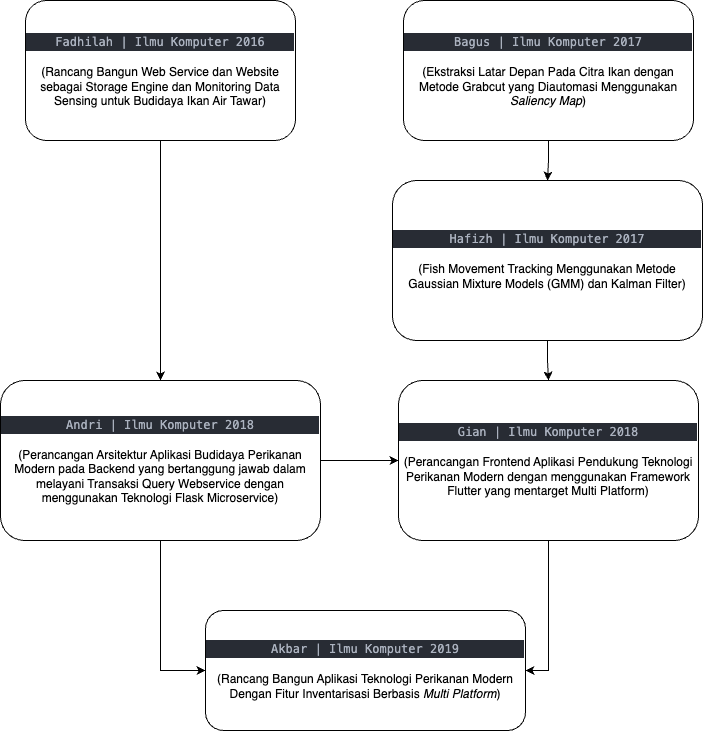
\includegraphics[width=0.7\textwidth]{gambar/research_tree.png}
	\caption{Diagram Alur Penelitian \textit{Aquaculture}}
\end{figure}

Pada diagram diatas, dapat dilihat urutan arah dari topik penelitian Aquaculture. Penelitian pertama kali dimulai oleh \citep{fadhil2021} dengan mengembangkan sebuah web service serta website yang berfungsi sebagai Storage Engine dan Monitoring Data Sensing untuk digunakan pada Budidaya Perikanan Air Tawar sebagai media penyimpanan data-data sensing dari sensor yang dikirimkan ke sistem serta memonitoringnya dalam bentuk table dan grafik real-time serta penelitian yang dilakukan oleh \citep{bagus2022} dengan tujuan untuk membangun sistem deteksi objek pada citra ikan dengan metode GrabCut yang telah diautomasi menggunakan \textit{saliency map}. 

Penelitian \citep{bagus2022} kemudian dilanjutkan oleh \citep{hafiz2021} yaitu merancang dan membangun sebuah sistem yang dapat melakukan pelacakan pergerakan ikan dengan menggunakan metode GMM dan Kalman Filter. Sementara penelitian \citep{fadhil2021} belum diterapkan pada aplikasi riset Aquaculture dalam waktu dekat sehingga penelitian yang dibuat oleh \citep{andri2022} dilakukan dengan membuat web service juga yang bertujuan untuk melayani transaksi query berupa monitoring budidaya perikanan yang dibarengi dengan penelitian \citep{gian2022} pada bagian perancangan \textit{frontend} sebagai pendukung pada aplikasi yang dikembangkan.

Dalam penelitian yang sudah berjalan ini, penulis mengembangkan penelitian yang dilakukan oleh \citep{andri2022} dan \citep{gian2022} dengan membuat fitur baru yaitu manajemen inventaris serta penentuan harga jual ikan dan penentuan upah pembudidaya ikan.

\section{Metode Penentuan Nilai Jual}

Dalam beberapa skenario, harga jual ditentukan oleh pedagang kepada pembudidaya. Harga ini dijamin lebih kecil dibanding harga retail, karena pedagang akan mengambil keuntungan dari itu. Jika dimisalkan T adalah harga jual minimum agar pembudidaya tidak rugi, $W_{feed}$ sebagai total pakan yang diberikan dan P adalah harga satuan pakan. Maka hubungan dari variabel-variabel tersebut adalah sebagai berikut.
\begin{equation}
    \begin{split}
		T
		&= W_{feed} \times P
    \end{split}
\end{equation}

Rumus ini didasari oleh konversi antara kilogram pakan menjadi pertambahan berat sebagian besar bervariasi tergantung pada kasus tertentu. Terlepas dari itu ditentukan oleh semakin tinggi asupan protein, maka semakin rendah tingkat konversinya. Jika konversi ini dikaitkan sebagai Food Conversion Ratio  (FCR) yang dimana $W_{fish}$ sebagai total berat dari semua ikan yang dipanen.
\begin{equation}
    \begin{split}
		FCR
		&= W_{feed } \div W_{fish}
    \end{split}
\end{equation}

Oleh karena itu, pembudidaya harus mencatat berapa banyak kilogram pakan yang diberikan sampai musim panen dari tiap kolam untuk menemukan nilai FCR-nya. Dalam masalah yang lebih kompleks, jika pakan memungkinkan datang dari berbagai sumber yang berhubungan dengan variasi asupan protein, FCR tidak dapat digunakan untuk menentukan hubungan antara jumlah pakan dan pertambahan berat.  Maka dari itu, sangat direkomendasikan untuk pembudidaya agar menggunakan satu sumber asupan protein tiap musim panen. Karena FCR sudah diketahui, selama musim panen berikutnya pembudidaya bisa memperkirakan berapa banyak pakan yang dibutuhkan untuk membuat ikan agar tumbuh sampai ukuran yang ditargetkan.
\begin{equation}
    \begin{split}
		W_{fish}
		&= W_{feed} \div FCR
    \end{split}
\end{equation}

Dengan itu bisa digunakan dalam mencari total jumlah pakan yang dibutuhkan untuk membuat ikan agar tumbuh sampai ukuran yang ditargetkan. 
\begin{equation}
    \begin{split}
		W_{feed}
		&= W_{fish} \times FCR
    \end{split}
\end{equation}

Jika persamaan 4 dikembangkan dengan memasukkan dua variabel yaitu $W_i$ sebagai berat ikan dan n sebagai jumlah ikan, maka persamaan akan menjadi seperti berikut.
\begin{equation}
    \begin{split}
		W_{fish}
		&= \sum_{i=1}^n \times W_i
    \end{split}
\end{equation}

Namun, menggunakan persamaan 5 akan mematikan tujuan dari persamaan 4, karena jika ingin menghitung pemakaian pakan diharuskan untuk menilai masing-masing ikan secara individu yang dimana itu tidak praktis. Jika menggunakan variabel $W_{af}$ sebagai rata-rata dari berat ikan, maka persamaan akan menjadi sebagai berikut.
\begin{equation}
    \begin{split}
		W_{af}
		&= \frac{\sum_{i=1}^n \times W_i}{n}
    \end{split}
\end{equation}

Sekarang dapat dengan mudah mencari perkiraan konsumsi pakan untuk musim panen berikutnya dengan persamaan,
\begin{equation}
    \begin{split}
		W_{feed}
		&= W_{af} \times n \times FCR
    \end{split}
\end{equation}


Jika persamaan 1 diupdate sehingga dapat ditemukan harga sesuai dengan persamaan,
\begin{equation}
    \begin{split}
		T_{unit}
		&= \frac{T}{n}
    \end{split}
\end{equation}

Persamaan itu juga merujuk pada jumlah perdagangan dalam kilogram, oleh karena itu
\begin{equation}
    \begin{split}
		k
		&= \frac{1kg}{W_{af}}
    \end{split}
\end{equation}

\begin{equation}
    \begin{split}
		T_k
		&= T_{unit} \times k
    \end{split}
\end{equation}

Sebagai contoh, dimisalkan mata uang yang digunakan adalah koin lalu FCR bernilai 1.5, ukuran target panen adalah 4 ikan per kilogram, di kolam terdapat 1000 ikan, dan harga pakan mencapai 10 koin.

Dari data tersebut, dapat diketahui $W_{af}$ = 1/4 kg, n = 1000. Karena itu, $W_{feed}$ bernilai 375 kg yang harus dipersiapkan. Selanjutnya, pembudidaya tidak bisa menjual semua hasil panen ikan seharga dibawah T = 3750 koin atau dibawah 15 koin per kilogram.

Persamaan 1 sampai 10 memungkinan jika FCR konstan dengan treatment yang sama dan asupan protein yang sama. Seperti yang sudah dilakukan diawal, pembudidaya harus mengandalkan satu sumber protein tetapi untuk mempertahankan hal ini sulit dilakukan. Karena itu, PER (Protein Efficiency Ratio) diketahui untuk menentukan rasio massa tubuh yang diperoleh dengan gram protein yang dikonsumsi. Disini variabel $P_{feed}$ mendefinisikan asupan gram protein.
\begin{equation}
    \begin{split}
		PER
		&= \frac{W_{fish}}{P_{feed}}
    \end{split}
\end{equation}

Pada formula tersebut, menggantikan $W_{feed}$ pada persamaan 2 dengan $P_{feed}$ akan memberikan bentuk variabel yang sama namun struktur variabel yang terbalik. Hal ini juga memberikan kemungkinan untuk mencampur beberapa sumber protein yang berbeda dengan formula berikut.
\begin{equation}
    \begin{split}
		PER
		&= \frac{W_{fish}}{P^1_{feed} + P^2_{feed} + \dots + P^k_{feed}}
    \end{split}
\end{equation}

\begin{equation}
    \begin{split}
		PER
		&= \frac{W_{fish}}{\sum_{i=1}^k \times P^i_{feed}}
    \end{split}
\end{equation}

Variabel k mengartikan jumlah dari sumber protein yang berbeda. Hal ini juga dapat dilakukan pada FCR dan T sebagai berikut.
\begin{equation}
    \begin{split}
		FCR
		&= \frac{\sum_{i=1}^k \times W^k_{feed}}{W_{fish}}
    \end{split}
\end{equation}
\begin{equation}
    \begin{split}
		T
		&= \sum_{i=1}^k \times W^k_{feed} \times P
    \end{split}
\end{equation}

Pada persamaan 15, hanya memodelkan harga jual minimum barang perikanan agar terhindar dari kerugian. Karena itu, untuk mendapatkan keuntungan diperlukan model yang baru. Disini variabel $T_p$ melambangkan dagangan yang memberikan keuntungan dan $F_g$ sebagai pendapatan pembudidaya.
\begin{equation}
    \begin{split}
		T_p
		&= T + F_g
    \end{split}
\end{equation}

$F_g$ merepresentasikan berapa banyak jam kerja yang dilakukan pembudidaya untuk membudidayakan ikan. Hal ini dapat dijelaskan lebih rinci dalam
\begin{equation}
    \begin{split}
		F_g
		&= D \times S
    \end{split}
\end{equation}

Dimana D mengartikan berapa banyak hari pembudidaya bekerja sampai musim panen dan S mengartikan upah yang mewakili pendapatan pekerjaan. Dalam berbudidaya, merupakan hal umum bagi pembudidaya ikan untuk menghabiskan waktu seharian penuh untuk mengembangkan dan memantau kolam, karena itu representasi hari lebih ideal. Sebab itu, pembudidaya yang lebih banyak menghabiskan waktunya sampai musim panen tiba harus mendapatkan pendapatan yang sesuai.

Persamaan 15 berlaku jika budidaya ikan membudidayakan ikan tradisional secara tradisional. Dalam sistem intensif aquaculture khususnya BFT, dibutuhkan variabel yang mewakili biaya tambahan yang dikeluarkan untuk penggunaan teknologi. Variabel ${C_i}$ merepresentasikan masing-masing biaya tambahan yang dikeluarkan dalam BFT untuk keseluruhan musim kawin.
\begin{equation}
    \begin{split}
		T
		&= \sum_{i=1}^k \times W^k_{feed} \times P + \sum_{i=1}^l \times C_i
    \end{split}
\end{equation}

Variabel $C_i$ dapat dijabarkan sebagai berikut.

\begin{itemize}
	\item $C_1$ = Bahan baku (termasuk pakan dan bahan budidaya)
	\item $C_2$ = Listrik (dihitung dalam per kolam)
	\item $C_3$ = Tenaga kerja (dihitung 3-5 jam / orang serta dibagi dengan jumlah kolam)
	\item $C_4$ = Benih ikan
\end{itemize}

Dalam menyimpan bahan baku pada inventaris, bahan baku tersebut akan mengalami penurunan karena bahan baku mempunyai masa kadaluarsa. Maka dari itu, dapat dimisalkan jika per bulan bahan baku tersebut mengalami penurunan kualitas sebesar 25\% dari harga belinya, maka dalam 4 bulan bahan baku tersebut akan kadaluarsa dan sudah tidak lagi berharga. Namun, skala penurunan tersebut bervariasi tergantung pada jenis bahan baku yang digunakan. Variabel $W_p$ mewakili harga dari bahan baku yang digunakan dan variabel $\alpha$ mewakili skala depresiasi per bulan dari bahan baku yang digunakan. Formula depresiasi dapat dibuat menjadi persamaan berikut.

\begin{equation}
    \begin{split}
		W_p
		&= W_p - \alpha \times W_p
    \end{split}
\end{equation}

\section{Tahapan Penelitian}

\begin{figure}[H]
	\centering
	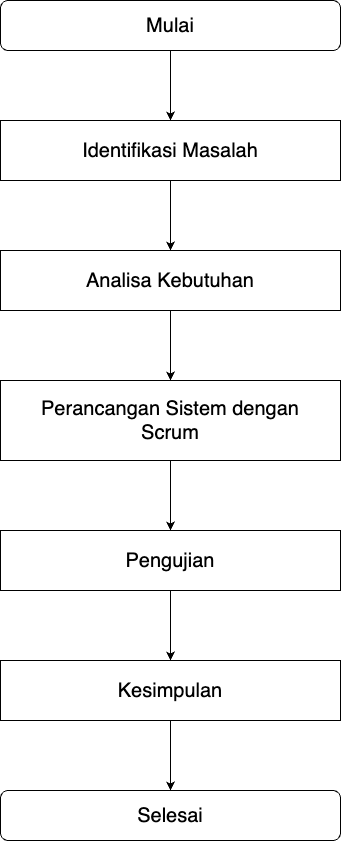
\includegraphics[width=0.35\textwidth]{gambar/tahapan_penelitian.png}
	\caption{Alur Tahapan Penelitian}
\end{figure}

Desain penelitian adalah alur yang dijalankan selama masa pengembangan aplikasi. Pada Gambar 3.2, terdapat desain penelitian yang digunakan dalam pembuatan aplikasi ini dengan metode Scrum.

% \section{Analisa Arsitektur Fitur}

% Pada penelitian aplikasi yang sudah dikembangkan sebelumnya, terdapat use case yang menjelaskan konsep dari aplikasi yang ada pada gambar dibawah ini.

% \begin{figure}[H]
% 	\centering
% 	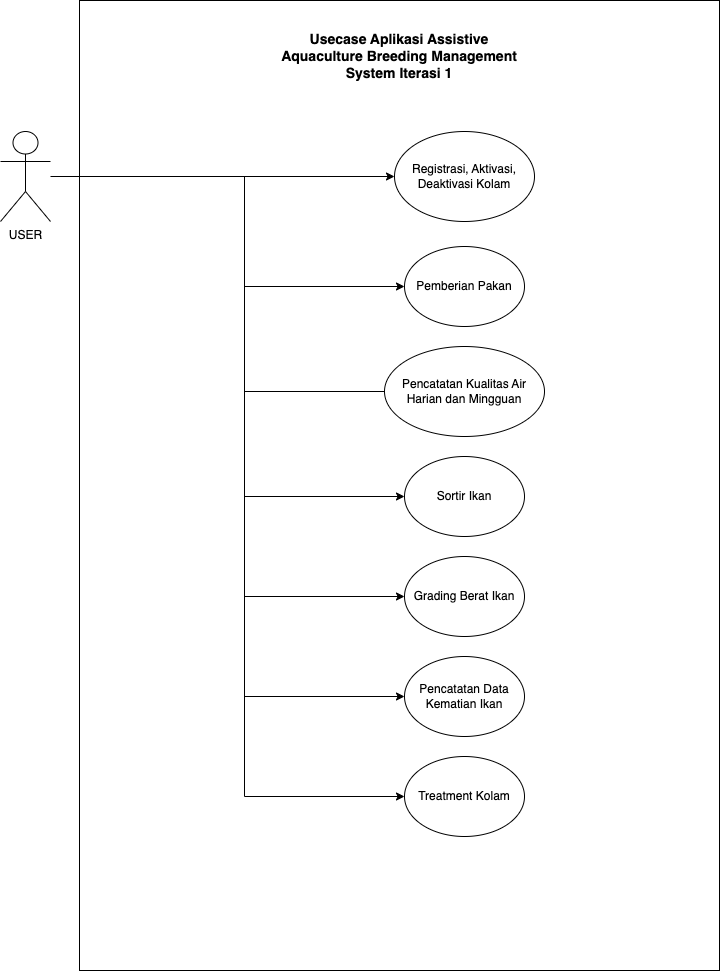
\includegraphics[width=0.8\textwidth]{gambar/usecase_iterasi_1.png}
% 	\caption{Use Case Fitur Aplikasi pada Iterasi 1}
% \end{figure}

% Dari diagram use case tersebut, terdapat dua jenis pengguna yaitu user dan admin. User dan admin memiliki fitur yang sama dalam aplikasi tersebut, yang membedakan antara user dan admin adalah skala prioritas dari aplikasi. Sisi admin memungkinkan pengguna dapat mengatur lebih banyak fitur yang ada pada aplikasi dan mendapatkan akses untuk mengatur user non-admin. Fitur yang disediakan aplikasi dijelaskan sebagai berikut.

% \begin{enumerate}
% 	\item \textbf{Registrasi, Aktivasi, Deaktivasi Kolam} = Fitur ini digunakan untuk mendaftarkan kolam yang akan dijadikan tempat budidaya ikan, kemudian fitur aktivasi dan deaktivasi kolam digunakan untuk mengontrol kolam yang sedang berjalan.
% 	\item \textbf{Pemberian Pakan} = Fitur ini digunakan untuk mencatat data pakan yang diberikan pada kolam ikan di budidaya yang sedang berlangsung.
% 	\item \textbf{Pencatatan Kualitas Air Harian dan Mingguan} = Fitur ini digunakan untuk mencatat kualitas air dari kolam di budidaya yang sedang berjalan dengan rentang waktu harian dan mingguan.
% 	\item \textbf{Sortir Ikan} = Fitur ini digunakan untuk mengatur perpindahan ikan ke kolam lain.
% 	\item \textbf{Grading Berat Ikan} = Fitur ini digunakan untuk mengatur ekosistem ikan berdasarkan berat agar mendapatkan keseragaman ukuran ikan dan meningkatkan efektivitas pemberikan pakan kepada ikan.
% 	\item \textbf{Pencatatan Data Kematian Ikan} = Fitur ini digunakan untuk mencatat angka kematian ikan jika terdapat ikan yang mati ketika budidaya sedang berjalan.
% 	\item \textbf{Treatment Kolam} = Fitur ini digunakan untuk melakukan pengaturan terhadap kolam ikan pada budidaya yang sedang berjalan.
% \end{enumerate}

\section{Analisa Kebutuhan}

Pada pengembangan aplikasi lanjutan ini, fitur yang ditambahkan adalah fitur manajemen inventaris serta fitur pembukuan. Fitur pencatatan inventaris merupakan fitur yang akan ada pada aplikasi yang berguna untuk para pembudidaya ikan mencatat semua hal yang berhubungan dengan budidaya perikanannya. Hal-hal yang dapat dicatat oleh pembudidaya pada fitur ini seperti bahan baku (termasuk pakan dan bahan budidaya), penggunaan listrik, benih, serta aset yang digunakan selama masa budidaya dilakukan.

Selain mencatat inventaris pada musim budidaya, fitur pencatatan inventaris ini juga dapat menentukan rekomendasi harga jual dari ikan yang dipanen oleh pembudidaya ikan berdasarkan perhitungan dari pengeluaran biaya selama musim budidaya berjalan. Beberapa fitur yang sudah ada di penelitian sebelumnya juga harus diperbarui dengan adanya manajemen inventaris ini seperti panen, pemberian pakan, sortir ikan, serta treatment kolam.

Kemudian untuk fitur pembukuan berguna untuk pembudidaya ikan melihat riwayat musim budidaya yang sudah mereka jalankan. Terdapat beberapa rincian yang ditampilkan seperti biaya pengeluaran sampai berapa total ikan yang terpanen pada musim budidaya tersebut.

Fitur-fitur tersebut dapat dibuat menjadi use case pada \textbf{Gambar 3.3}. Pada use case tersebut, font warna hitam merupakan fitur yang sudah ada pada penelitian sebelumnya yang tidak berubah dan font warna cokelat merupakan fitur sebelumnya yang akan diperbarui pada penelitian ini. Sementara itu, untuk font warna hijau merupakan fitur baru yang akan tersedia pada aplikasi dan dikembangkan pada penelitian ini.

\begin{figure}[H]
	\centering
	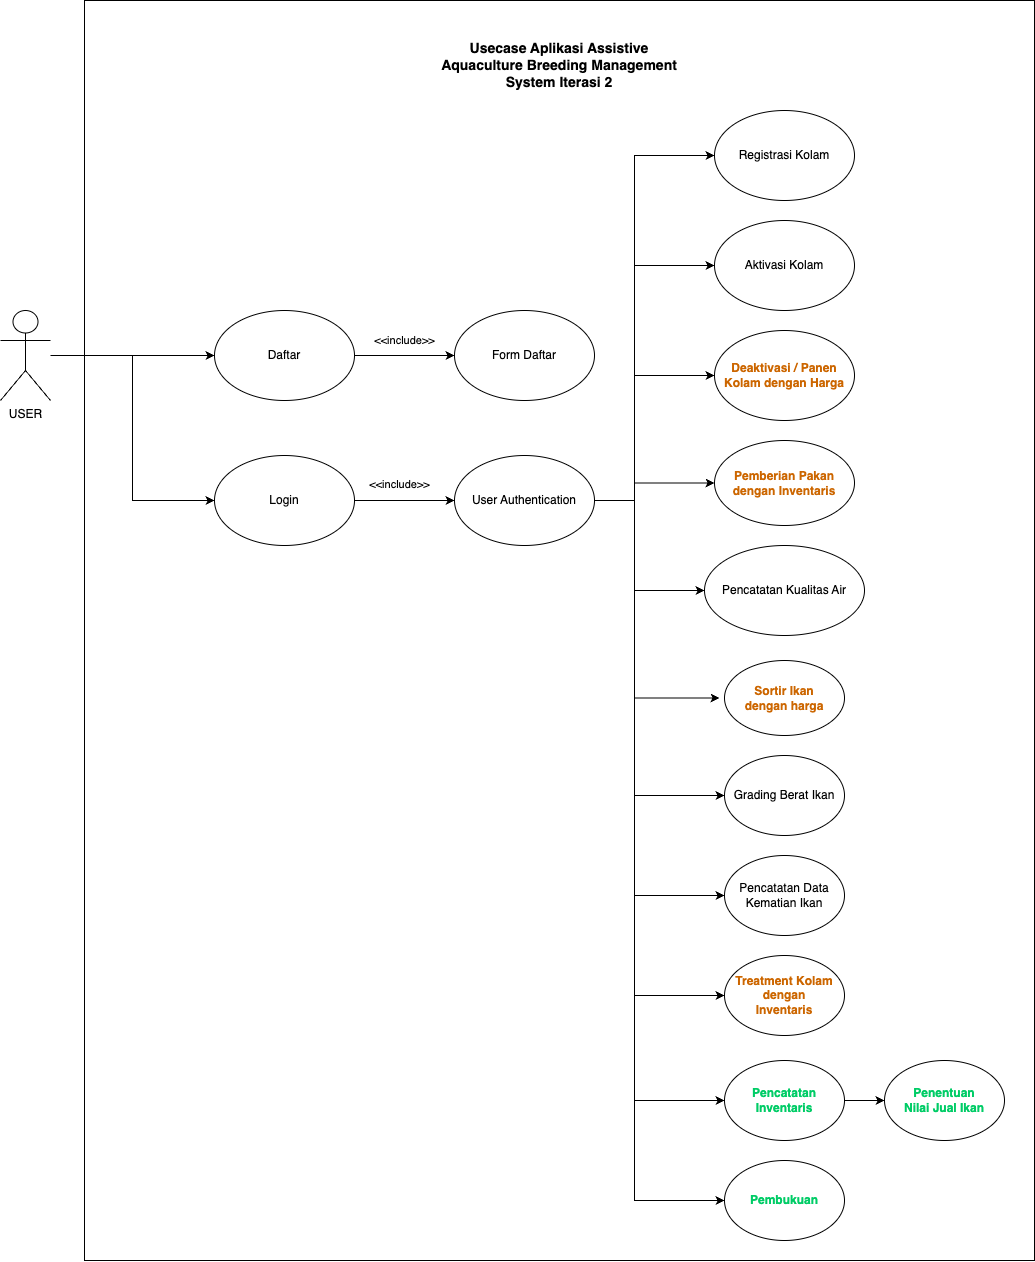
\includegraphics[width=0.9\textwidth]{gambar/usecase_iterasi_2.png}
	\caption{Use Case Aplikasi}
\end{figure}

\section{Perancangan Sistem}

Pada aplikasi yang akan dibuat pada penelitian ini dikembangkan dengan metode Scrum. Beberapa komponen scrum seperti product backlog, sprint backlog, daily sprint, serta daily meet digunakan agar terwujudnya ketertiban dalam masa pengembangan aplikasi. Berikut penjelasan dari masing-masing elemen yang ada pada metode Scrum.

\begin{figure}[H]
	\centering
	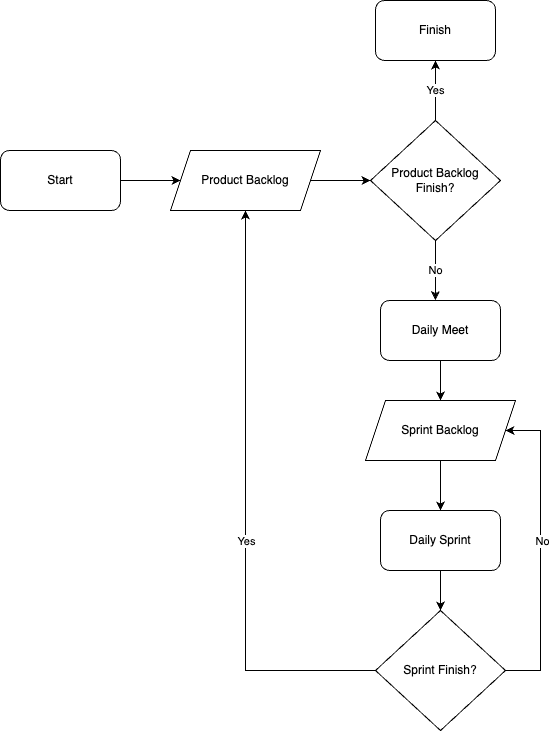
\includegraphics[width=0.8\textwidth]{gambar/scrum.png}
	\caption{Tahapan Perancangan Sistem dengan Metode Scrum}
\end{figure}

\begin{enumerate}
	\item Product Backlog
	
	Product Backlog adalah tugas-tugas yang \textbf{akan} dijalankan pada penelitian dan hal yang pertama kali dilakukan sebelum memulai riset. Daftar tugas yang ada pada Product Backlog ini akan dipindahkan pada Sprint Backlog tergantung pada skala prioritas dari task itu sendiiri. Berikut adalah tabel dari Product Backlog yang sudah berjalan.

	\begin{table}[H]	
		\begin{center}
			\caption{Tabel Product Backlog}
			\label{tab:table5}
			\begin{tabular}{|c|m{17em}|c|c|}
			\hline
			\textbf{No} & \textbf{Stories} & \textbf{Sprint} & \textbf{Status} \\
			\hline
			1 & Pencatatan inventaris & 1, 2 & On Progress \\
			\hline
			2 & Depresiasi aset dalam inventaris & - & Uncomplete \\
			\hline
			3 & Pemberian pakan yang terkoneksi dengan inventaris & - & Uncomplete \\
			\hline
			4 & Treatment kolam yang terkoneksi dengan inventaris & - & Uncomplete \\
			\hline
			5 & Sortir termasuk harga nilai jual ikan & - & Uncomplete \\
			\hline
			6 & Panen termasuk harga nilai jual ikan & - & Uncomplete \\
			\hline
			7 & Pembukuan pencatatan pengeluaran per musim budidaya & - & Uncomplete \\
			\hline
			\end{tabular}
		\end{center}
	\end{table}	

	\item Sprint Backlog
	
	Sprint Backlog adalah daftar tugas yang \textbf{harus} dijalankan selama masa Sprint berlangsung. Tugas yang ada pada Sprint Backlog bersifat fleksibel seiring dengan berjalannya Sprint. Berikut merupakan tabel dari Sprint Backlog yang sudah berjalan.

	\begin{table}[H]	
		\begin{center}
			\caption{Tabel Sprint 1 Backlog}
			\label{tab:table6}
			\begin{tabular}{|c|c|m{13em}|c|}
			\hline
			\textbf{No} & \textbf{Stories} & \textbf{Task} & \textbf{Status} \\
			\hline
			1 & \multirow{2}{10em}{Fitur pencatatan inventaris} & - Membuat skema database dari pencatatan inventaris & Complete \\
			&  & - Membuat mockup dari fitur inventaris & Complete \\
			\hline
			\end{tabular}
		\end{center}
	\end{table}

	\begin{table}[H]	
		\begin{center}
			\caption{Tabel Sprint 2 Backlog}
			\label{tab:table7}
			\begin{tabular}{|c|c|m{13em}|c|}
			\hline
			\textbf{No} & \textbf{Stories} & \textbf{Task} & \textbf{Status} \\
			\hline
			1 & \multirow{2}{10em}{Fitur pencatatan inventaris} & - Membuat alur UI/UX dari design aplikasi & Complete \\
			&  & - Mengupdate skema database serta integrasinya pada inventaris & Complete \\ 
			% &  & -  & Complete \\ 
			\hline
			\end{tabular}
		\end{center}
	\end{table}

	\item Sprint
	
	Progres sprint dilaksanakan ketika list task pada sprint backlog sudah disepakati bersama. Periode pengerjaan sprint bervariasi tergantung pada kesulitan task dari sprint backlog tersebut.

	\begin{enumerate}
		\item \textbf{Sprint 1}
		
		Sprint 1 dilaksanakan pada tanggal 15 Februari 2023 - XX Maret 2023. Pada sprint ini mengerjakan tugas yang ada pada Sprint 1 Backlog di Tabel 3.2.

		Berikut merupakan skema database yang mewakili fitur inventaris dapat dilihat pada Gambar 3.4 berikut.
		
		\begin{figure}[H]
			\centering
			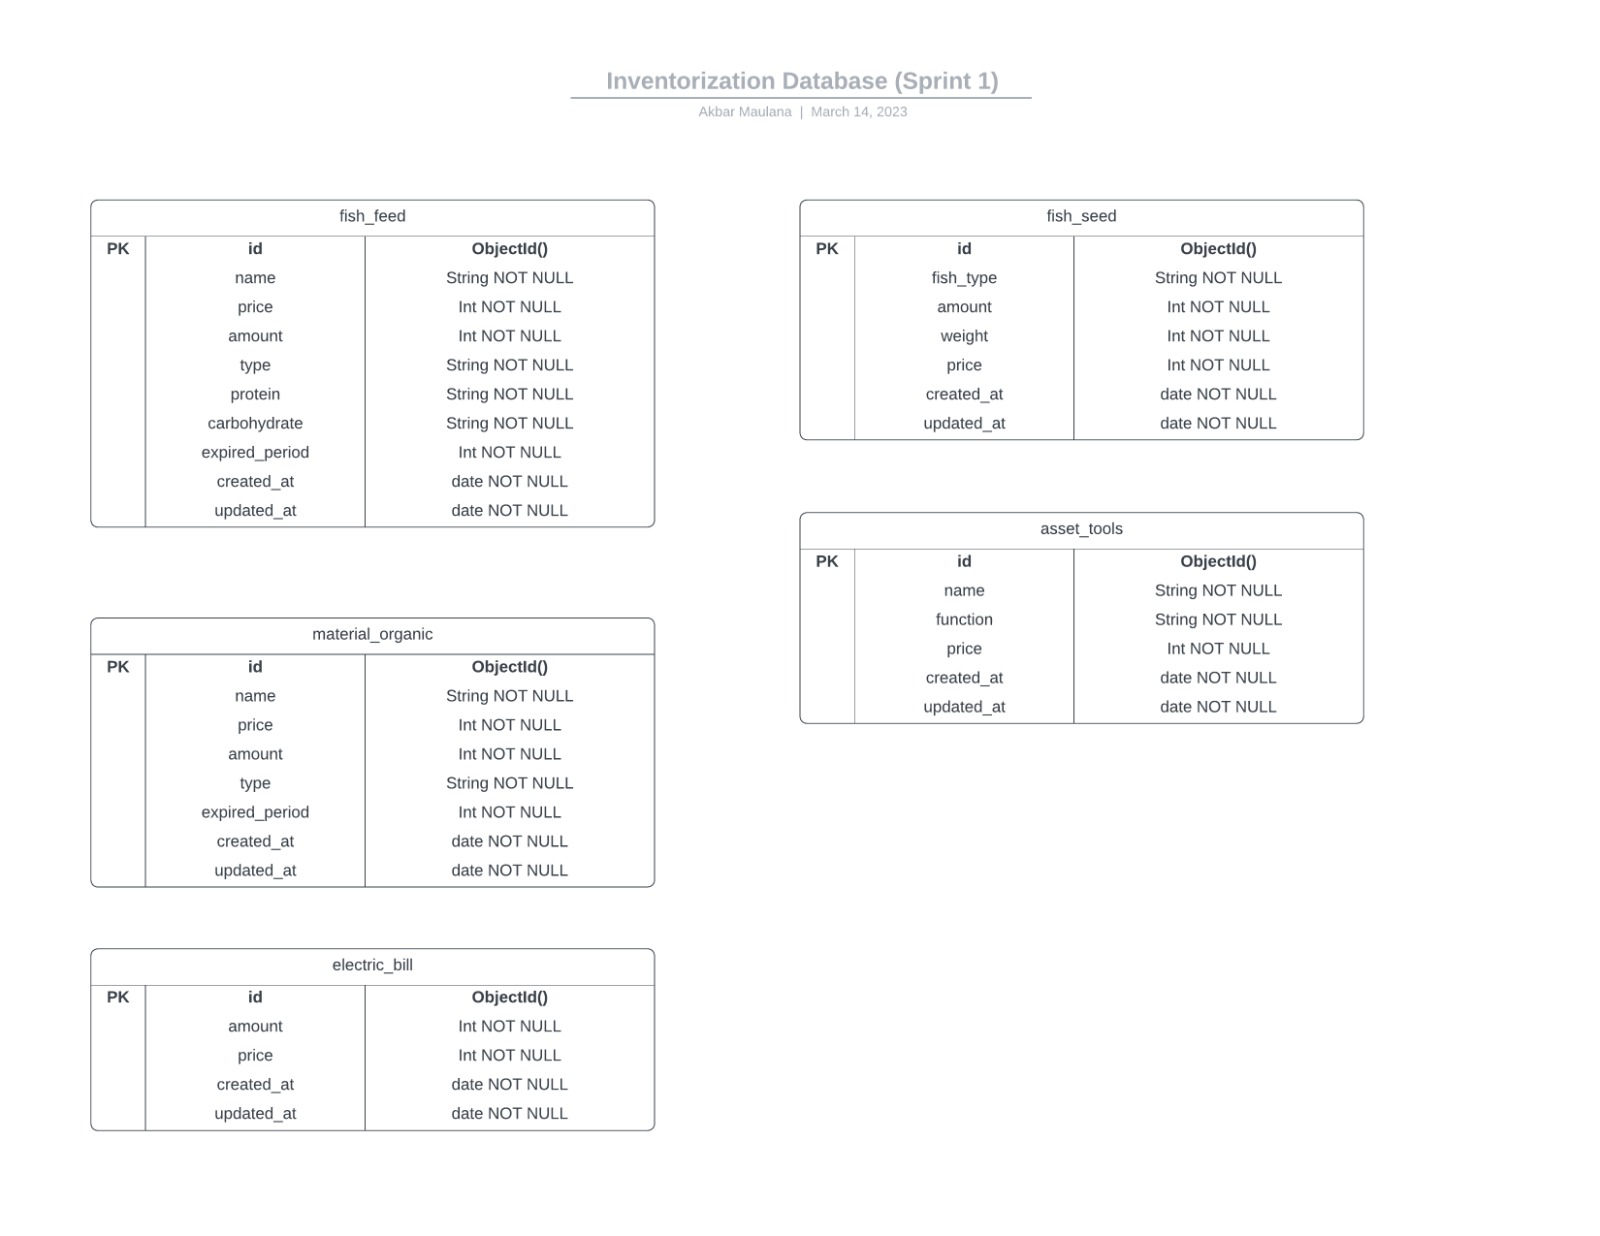
\includegraphics[width=1\textwidth]{gambar/sprint1/sprint1_inventaris_database.jpeg}
			\caption{Skema Database Fitur Inventaris}
		\end{figure}
	
		Dari skema database tersebut, terdapat lima opsi kategori inventaris yang sudah dijelaskan sebelumnya. Pada skema database ini, masing-masing kategori memiliki kebutuhan yang berbeda antara lain.
	
		\begin{enumerate}
			\item fish\_feed (Pakan Ikan)
			\item material\_organic (Bahan Organik)
			\item electric\_bill (Tagihan Listrik)
			\item fish\_seed (Benih Ikan)
			\item asset\_tools (Peralatan)
		\end{enumerate}
	
		Dalam tabel database tersebut, pada kolom pertama terdapat jenis \textit{key} yang dijadikan patokan dalam tabel database tersebut. Kemudian kolom kedua dan ketiga merupakan hubungan antara nama data dan tipe data yang mewakili nama data tersebut.
	
		Setelah skema database dari inventaris telah dibuat, tabel-tabel database tersebut harus diintegrasikan dengan skema database sebelumnya untuk menyesuaikan kebutuhan fitur yang akan dibuat nantinya. Berikut merupakan skema database yang telah diintegrasikan dengan skema database dari inventaris dapat dilihat pada Gambar 3.5.
	
		\begin{figure}[H]
			\centering
			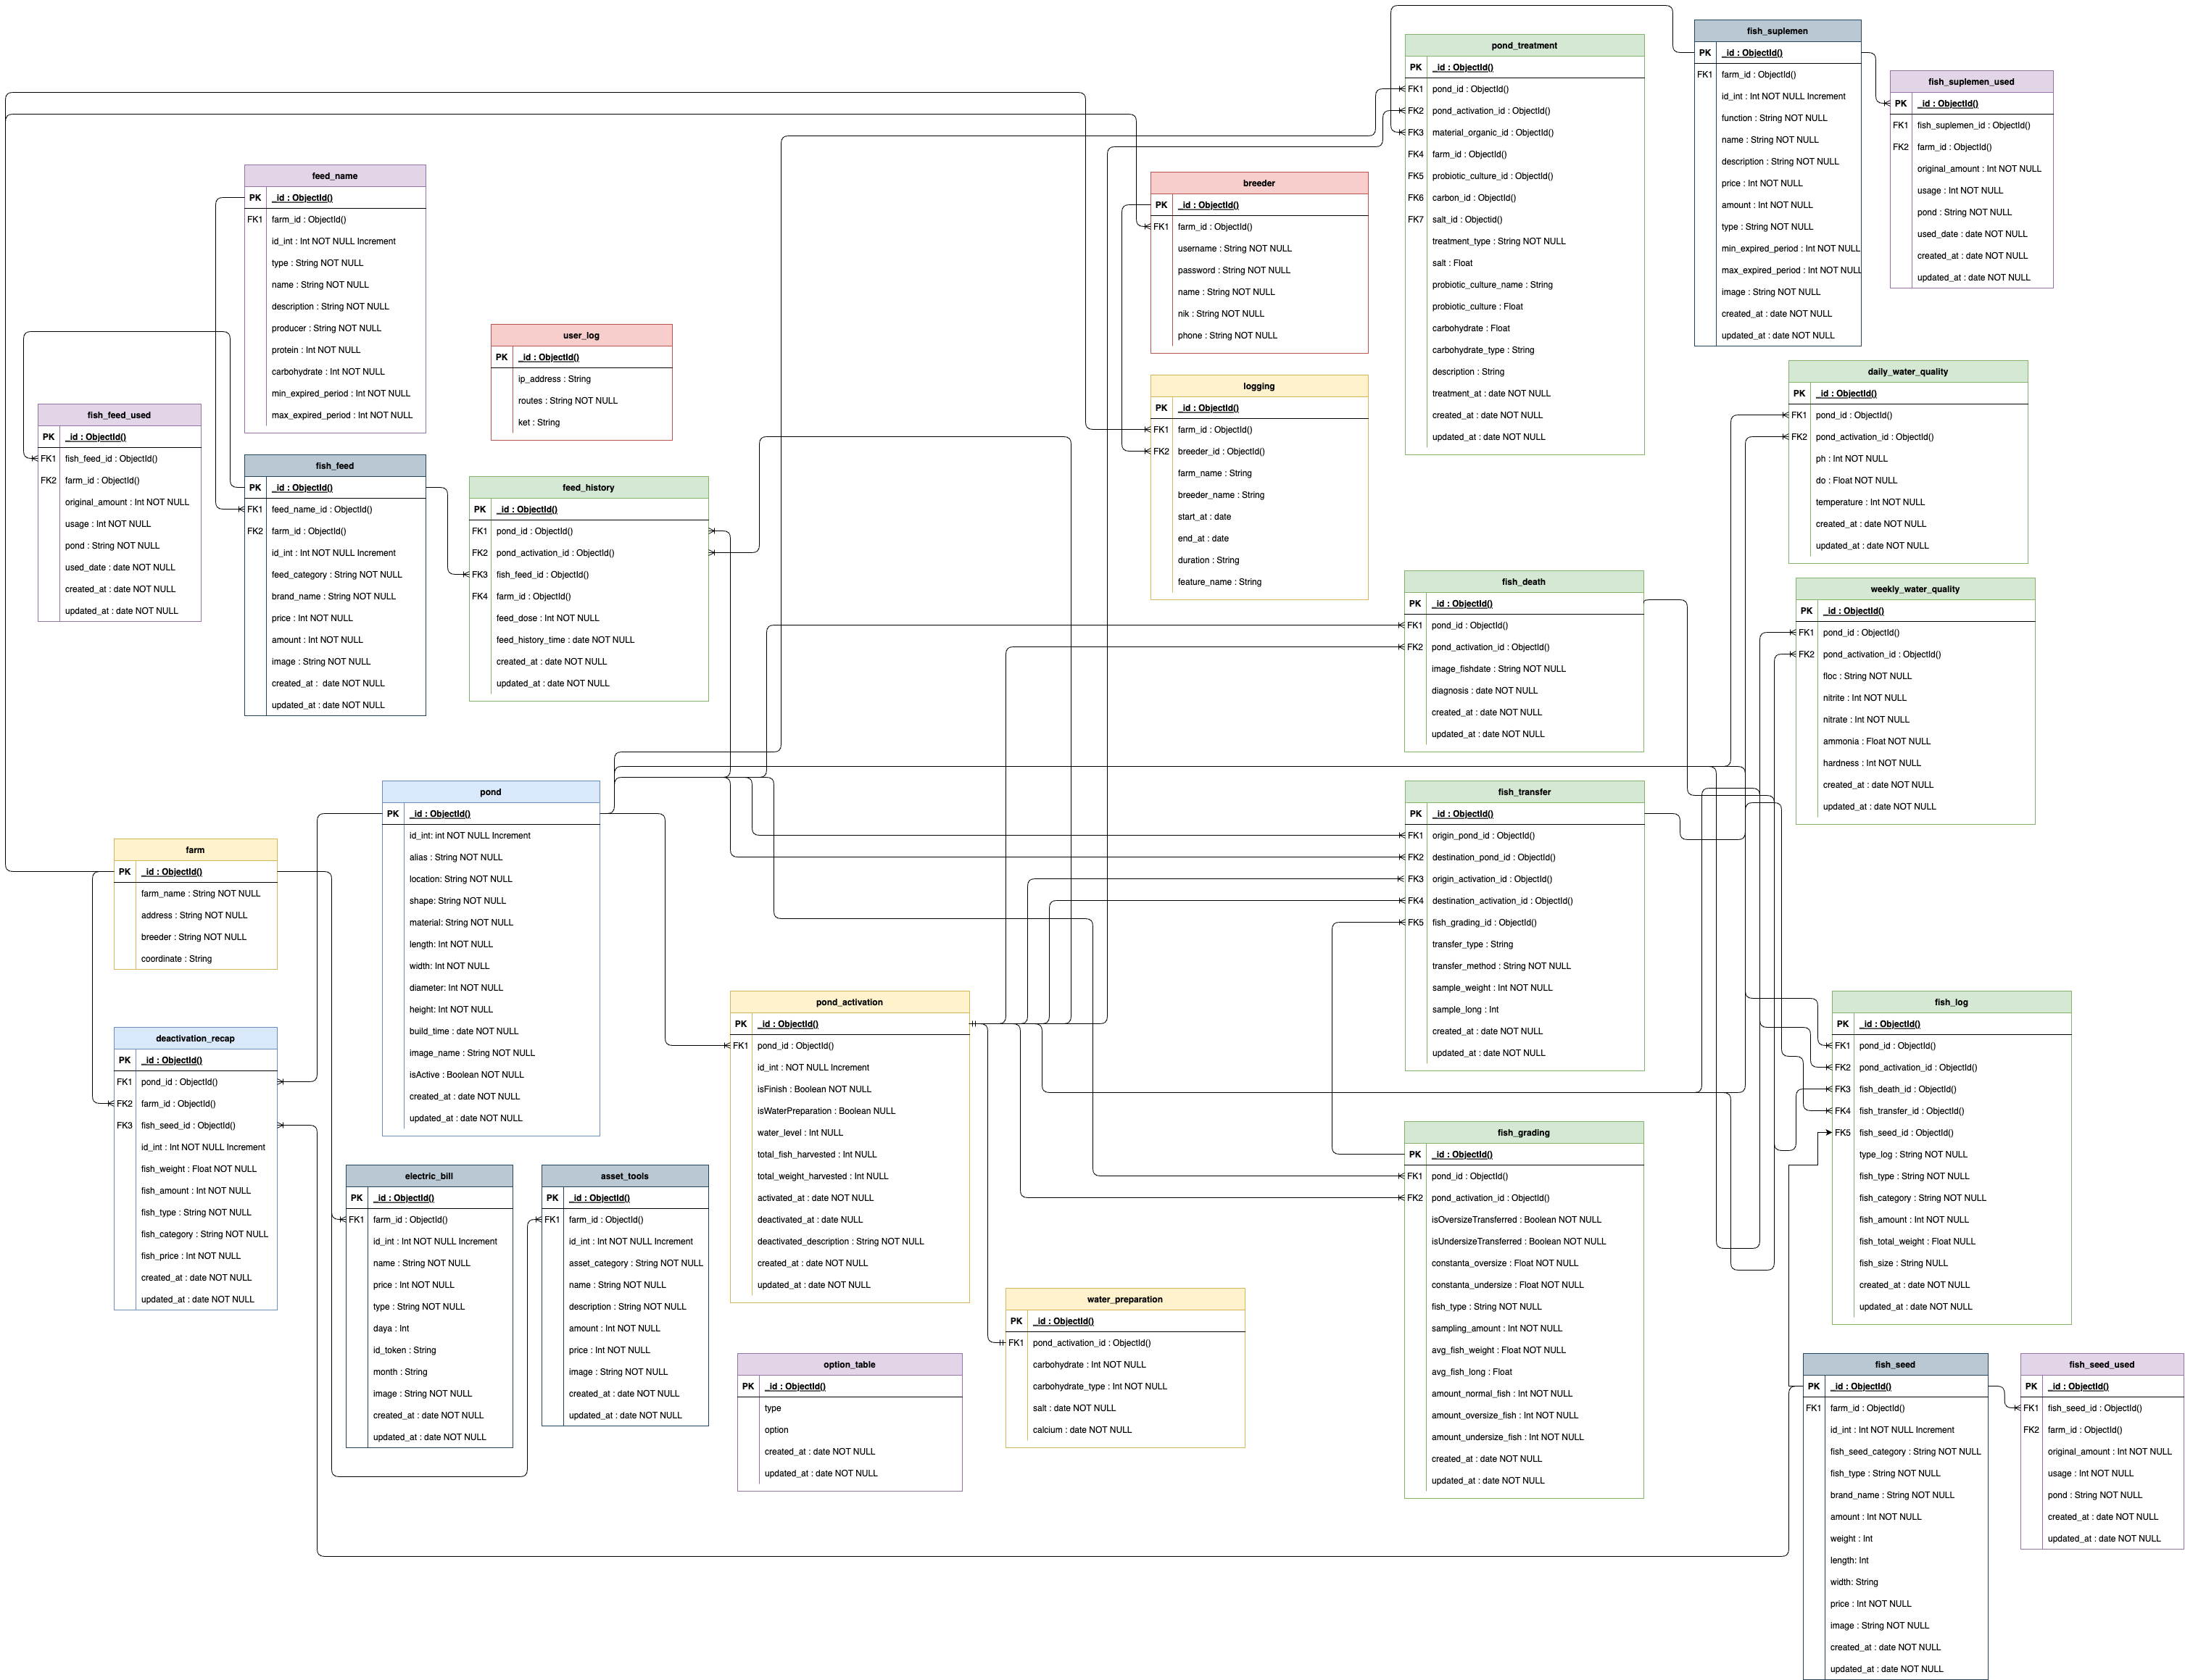
\includegraphics[width=1\textwidth]{gambar/sprint1/sprint1_skema_database.png}
			\caption{Integrasi Skema Database Inventaris dengan Skema Database Iterasi 1}
		\end{figure}

		\item \textbf{Sprint 2}
		
		Dalam membuat mockup design ini, 
		
		Berikut merupakan mockup dari fitur inventaris berdasarkan skema database yang sudah dibuat sebelumnya.
	\end{enumerate}
	
	\item Sprint Review
	
	Setelah Sprint berjalan, setiap minggunya diadakan meet bersama tim untuk melaksanakan Sprint Review yang bertujuan untuk melaporkan perkembangan Sprint baik itu proses ataupun hambatan selama pengerjaan Sprint.
	
	\item Deploy Sistem
	
	Ketika semua task sprint yang ada di sprint backlog selesai, maka aplikasi akan di deploy untuk dijalankan pengujian pada aplikasi. Pengujian aplikasi ini dilakukan dengan menggunakan Unit Testing dan User Acceptance Test (UAT).
	
\end{enumerate}

\section{Pengujian}



% \subsection*{Daily Scrum}

% Daily Scrum merupakan kegiatan rutin tiap minggu yang dilaksanakan dengan Scrum Master. Kegiatan ini dilakukan untuk reporting progres tugas yang dijalankan selama masa Sprint berlangsung kepada Scrum Master. Scrum Master bertugas untuk memberikan feedback saat Daily Scrum berlangsung.

% \subsection*{Sprint Review dan Sprint Restropective}

% Sprint Review dan Sprint Restropective adalah kegiatan mengulas kembali tugas yang sudah dikerjakan pada saat durasi Sprint berlangsung. Kegiatan ini juga merupakan kegiatan menentukan tugas yang berhasil dan tidak berhasil selama Sprint berlangsung
% \addcontentsline{toc}{chapter}{LAMPIRAN}
\appendix
\chapter {Transkrip Percakapan}
\begin{flushleft}
Hari: Rabu
\linebreak
Tanggal: 15 Maret 2023
\linebreak
PL: Penulis
\linebreak
KL: Klien (Pemilik Farm)
\linebreak
\linebreak
PL: Sistem apa yang akan di buat?
\linebreak
KL: Kita akan membuat sistem inventaris pada budidaya perikanan untuk penentuan harga jual minimum ikan
\linebreak
PL: Apa saja requirement dan fitur yang dibutuhkan oleh sistem ini?
\linebreak
KL: Fitur utama yang harus ada adalah sistem inventaris benih, inventaris pakan, inventaris suplemen, inventaris listrik, dan inventaris aset
\linebreak
PL: Bagaimana cara menentukan harga jual minimum ikan dari sistem inventaris tersebut?
\linebreak
KL: Dengan cara menghitung pengeluaran benih, pakan, suplemen, aset serta pengeluaran listrik per kolam aktif selama musim budidaya berjalan. Kemudian, pengeluaran tersebut akan dibagi dengan total ikan ketika masa panen tiba.
\linebreak
PL: Apakah dengan masuknya inventaris aset akan mempengaruhi nilai jual ikan per musim panen?
\linebreak
KL: Dengan masuknya harga aset kedalam perhitungan, harga ikan otomatis akan menjadi tinggi. Untuk itu, harga aset dibagi dengan 5 tahun masa pemakaian karena masa aset dalam inventaris bisa berlangsung lama. Dalam kasus ini diubah menjadi 60 bulan karena musim panen bisa dilakukan tiap bulan.
\linebreak
PL: Dimulai dari manakah pengerjaan fitur-fitur tersebut?
\linebreak
KL: Dimulai dari inventaris benih
\end{flushleft}

%-----------------------------------------------------------------
%Disini akhir masukan Bab
%-----------------------------------------------------------------


%-----------------------------------------------------------------
% Disini awal masukan untuk Daftar Pustaka
% - Daftar pustaka diambil dari file .bib yang ada pada folder ini
%   juga.
% - Untuk memudahkan dalam memanajemen dan menggenerate file .bib
%   gunakan reference manager seperti Mendeley, Zotero, EndNote,
%   dll.
%-----------------------------------------------------------------
\bibliography{daftar-pustaka}
\bibliographystyle{myapalike}
\addcontentsline{toc}{chapter}{DAFTAR PUSTAKA}
%-----------------------------------------------------------------
%Disini akhir masukan Daftar Pustaka
%-----------------------------------------------------------------


\end{document}